              %******************************************%
              %                                          %
              % Template standard per la Tesi di Laurea  %
              %            di Stefano Bianchi            %
              %                                          %
              %         versione: 27 marzo 2014          %
              %                                          %
              %******************************************%
       
% Se si vuole stampare su entrambi i lati, porre la dicitura 'twoside'
% tra i parametri documentclass
\documentclass[a4paper,11pt,oneside,openany]{book}

\usepackage[english,italian]{babel}

\usepackage[utf8]{inputenc} % Consente l'uso dei caratteri accentati italiani
\usepackage[T1]{fontenc} % Consente l'uso di caratteri speciali appartenenti in genere ad alfabeti non inglesi

\usepackage{fancyhdr} % Consente il rendering della copertina

\usepackage{graphicx} % Consente l'inserimento delle figure nel documento

%----------------PERSONAL ADDITION-------------
\usepackage{tikz}
\usetikzlibrary{arrows.meta, positioning, calc, shapes}
\usepackage{tabularx}
\usepackage{booktabs}
\usepackage{url}
\usepackage{pdflscape} %things need to be landscaped
%----------------END PERSONAL ADDITION-------------

\usepackage{subfigure} % Consente l'inserimento di sottofigure

\usepackage{tabularx} % Consente l'uso di funzionalità aggiuntive alle tabelle
\usepackage{longtable} % Consente la scrittura delle tabelle su più pagine

\usepackage[titletoc]{appendix} % Consente di porre le appendici in indice

\usepackage{float} % Necessario per inserire immagini flottanti

\usepackage{fancyvrb} % Consente l'utilizzo di finestre Verbatim (testo cche si vuole porre così com'è, senza formattazione alcuna) all'interno di una cornice

\usepackage{amsmath} % Consente l'uso di funzioni aggiuntive per le formule
\numberwithin{equation}{section}

\usepackage{hyperref} % Indice degli argomenti e rimandi cliccabili, per una navigazione più comoda all'interno del file

\usepackage{lipsum} % Consente di inserire testo fittizio all'interno della tesi. Inutile in fase di scrittura della tesi. Eliminare questa dicitura e tutte le diciture \lorem all'interno del testo.

% Per inserire i contenuti, riferirsi ai file relativi e segnati tra parentesi graffe nei parametri \input


\newcommand{\revAC}[1]{\textcolor{violet}{AC: #1}}
\newcommand{\revMT}[1]{\textcolor{magenta}{SM: #1}}

\newcommand{\add}[1]{\textcolor{blue}{#1}}
\newcommand{\remove}[1]{\textcolor{red}{\sout{#1}}}

%*******************************************************
% Impostazioni della singola pagina e della copertina
%*******************************************************
\hypersetup{ % Visualizzazione dei collegamenti cliccabili
    colorlinks,
    citecolor=black,
    filecolor=black,
    linkcolor=black,
    urlcolor=black
}

% Imposta l'intestazione delle pagine
\fancyhf{}
\pagestyle{fancy}
\lhead{}
\chead{\leftmark}
\rhead{}
\lfoot{}
\cfoot{}
\rfoot{\thepage}

%*******************************************************
% Copertina
%*******************************************************
% Imposta la copertina
% Non modificare questa parte
\usepackage[some]{background}
\SetBgScale{1}
\SetBgContents{

\includegraphics[scale=1]{img/units_logo.pdf}}
\SetBgColor{gray}
\SetBgAngle{0}
\SetBgOpacity{0.07}
% Non modificare questa parte

\begin{document}
% Titolo della tesi e autore
\title{Development and implementation of a feedback system for synchrotron x-ray beamline control based on the peak intensity of the photon beam}
\author{Matteo Pillinini}
\pagenumbering{roman}
\begin{titlepage}
    \begin{center}
    % Insert the background here (front page)
    \BgThispage
    {\LARGE {\bfseries UNIVERSIT\`A DEGLI STUDI DI TRIESTE \\}}
    \vspace{.5cm}
    {\Large {\bfseries Dipartimento di Ingegneria e Architettura \\}}
    \vspace{1cm}
    
\includegraphics[width=6cm,height=6cm]{img/units_logo.pdf}\\[1.5cm]

    {\LARGE
        Laurea Magistrale in Ingegneria Informatica \\
    }
    \vspace{1cm}
    {\LARGE 
        {\bfseries Reverse engineering per la decodifica di filmati di videosorveglianza in formato proprietario}
    }
    \vspace{1cm}

    % Ricordarsi di aggiornare la data prima di inviare in stampa il documento :)
    {\large \today \\
    }

    % Tabella per inserire i nomi del laureando, del relatore e dell'eventuale correlatore nel modo migliore all'interno della pagina
    \vfill
    \begin{table}[h]
        {\large
            \begin{tabular}{c c c c r c c | c c l}
                & & & & Laureando & & & & & Relatore \\
                & & & & \bfseries Matteo Pillinini & & & & & \bfseries Prof. Martino Trevisan \\ % Modificare il nome del laureando
                & & & & & & & & & \\
                & & & & & & & & & Correlatori \\ % Nel caso in cui non si ha il correlatore,
                & & & & & & & & & \bfseries Prof. Alberto Carini \\ % eliminare queste due righe
                & & & & & & & & & \bfseries Paolo Scarbolo \\ % eliminare queste due righe
                & & & & & & & & & \bfseries Borut Brecelj \\ % eliminare queste due righe
            \end{tabular}
        }
    \end{table}
    Anno Accademico 2026/2027
    \end{center}
\end{titlepage}


%*******************************************************
% Dedica
%*******************************************************
% Non modificare questa parte
\phantomsection
\thispagestyle{empty}
\vspace*{3cm}
% Non modificare questa parte

\begin{center}
Così tra questa \\
immensità s'annega il pensier mio: \\
e il naufragar m'è dolce in questo mare. \\
--- Giacomo Leopardi -- da \emph{L'infinito} ---
\end{center}

\medskip

\begin{center}
\hfill \emph{Dedica 1} \\
\hfill \emph{Dedica 2} \\
\hfill \emph{...} \\
~ \\
\hfill \emph{Altre frasi} \\
\hfill \emph{da dedicare} \\
\hfill \emph{alle persone care} \\
\end{center}
	
\frontmatter

%*******************************************************
% Sommario
%*******************************************************
\chapter{Sommario}

Le linee di luce di sincrotrone richiedono un flusso di fotoni stabile per garantire misurazioni sperimentali affidabili.
Durante gli esperimenti disturbi come la deriva termica e l'attrito meccanico possono influenzare i componenti della linea di fascio, in particolare il monocromatore a doppio cristallo (DCM), spostando il suo punto di lavoro dal picco della rocking curve, dove il flusso di fotoni è massimo.
Il sistema BEST (Beamline Enhanced Stabilization Technology), sviluppato da ELS Instruments, fornisce già il controllo della posizione del fascio a un determinato setpoint, ma non è in grado di seguire il picco di intensità.
Questa tesi presenta un sistema di controllo per il tracciamento del picco di intensità integrato nel sistema BEST.
La soluzione implementata sovrappone un piccolo segnale sinusoidale all'attuatore piezoelettrico che muove il monocromatore.
Il gradiente di intensità viena estratto ed elaborato da una catena digitale composta da un filtro passa-banda, una demodulazione sincrona, un filtro passa-basso e un controllore Proporzionale-Integrale-Derivativo (PID).
Portando il gradiente a zero, il sistema sposta il monocromatore verso il picco di intensità, indipendentemente dal suo valore.

L'implementazione ha richiesto modifiche a diverse parti del sistema BEST: la logica FPGA, il firmware in esecuzione sul processore soft-core integrato e l'interfaccia grafica locale.
Inoltre, poiché una corretta demodulazione richiede la conoscenza del ritardo di fase introdotto dall'intero sistema, è stata implementata una procedura di calibrazione iniziale per stimarlo a partire dalle componenti in fase e in quadratura (I/Q) del segnale mediante un arcotangente a quattro quadranti.
Il sistema è stato validato in un ambiente di simulazione Software-in-the-Loop (SIL), che ha permesso di testare il software implementato in diverse condizioni operative e dinamiche della rocking curve.
I risultati della simulazione hanno dimostrato la capacità del sistema di posizionare con precisione il monocromatore sul picco di intensità.
Nel complesso, questo lavoro estende il sistema BEST esistente con una capacità di feedback aggiuntiva, combinando la stabilizzazione della posizione del fascio con il tracciamento in tempo reale del picco d'intensità.

\chapter{Summary}

Synchrotron beamlines requires a stable photon flux to ensure reliable experimental measurements.
During experiments, especially long-duration ones, disturbances like thermal drift and mechanical friction, 
can affect beamline components, in particular the double crystal monochromator (DCM), shifting its working point away from the peak of the rocking curve, where photon flux is at its maximum.
The BEST (Beamline Enhanced Stabilization Technology) system, developed by ELS Instruments, already provides beam position control at a given setpoint, but cannot track the intensity peak.
This thesis presents the design, implementation and validation of a control system for peak intensity tracking integrated into the BEST system.
The implemented solution adds a small sinusoidal dither signal on the piezoelectric actuator that moves the monochromator.
The intensity gradient is extracted by a digital pipeline composed of a band-pass filter, synchronous demodulation, low-pass filter and a Proportional-Integral-Derivative (PID) controller.
By driving the gradient to zero, the system moves the monochromator towards the intensity peak, regardless of its value.

The implementation require modifications on several parts of the BEST system: the FPGA logic, the firmware running on the embedded soft-core processor, and the local GUI used for data visualization and system configuration.
Additionally, since correct demodulation requires knowledge of the phase delay introduced by the whole system, an initial calibration procedure has been implemented to estimate it from the in-phase and quadrature (I/Q) components of the signal by means of a four-quadrant arctangent.
The system has been validated in a Software-in-the-Loop (SIL) simulation environment, which made it possible to test the implemented software under different operating conditions and rocking curve dynamics.
The simulation results have shown the system ability to accurately position the monochromator at the intensity peak.
Overall, this work extends the existing BEST system with an additional feedback capability, combining beam position stabilization with real-time peak intensity tracking.

%*******************************************************
% Indice
%*******************************************************
\tableofcontents

%*******************************************************
% Introduzione
%*******************************************************
% Non modificare questa parte
\renewcommand{\chaptermark}[1]{\markboth{\MakeUppercase{\ #1}}{}}
% Non modificare questa parte



%*******************************************************
% Capitoli
%*******************************************************
\mainmatter

% Non modificare questa parte
\renewcommand{\chaptermark}[1]{\markboth{\MakeUppercase{\chaptername\ \thechapter.\ #1}}{}}
% Non modificare questa parte

% Inserire tutti i capitoli necessari. Si possono inserire tutti i capitoli
% all'interno di un singolo file .tex oppure un file .tex per ogni capitolo.

\chapter{Introduction}

\section{Particle Accelerators}

Particle accelerators are widely used in scientific research; they are facilities where a variety of experiments can be performed, including some using photon beams.
Experiments involving photon beams generally involve using the beam to strike a target material or sample to study its properties.
There are two main architectures for building particle accelerators:

\begin{itemize}
    \item linear accelerators (in-line).
    \item circular accelerators (synchrotrons).
\end{itemize}

A synchrotron is compose by different parts:

\begin{itemize}
    \item Linear accelerator: This is where the electrons begin their journey by acquiring velocity near the speed of light.
    \item Booster ring: After the linear accelerators, the electrons end up in a small ring where they gain energy until a threshold.
    \item Storage ring: After reaching the threshold energy, the electrons are injected into the storage ring where they maintain their energy for a long time.
\end{itemize}

The storage ring is composed by multiple straight segments, this imply the presence of angles between them.
The beam of electrons is steered by bending magnets from one segment to the other and by doing this they emit synchrotron radiation photons.
In this way is possible to route the photons into experimental stations called beamlines.
The beam need to be positioned correctly during the experiments and keep it in the right position.
Beam position monitors (BPMs) are used to locate the beam, they are minimally invasive type of device.
Once the position is known, a control system can be used to adjust the position of the beam so that it is at the target location.
The control system is able to modify the position of the beam by acting on the piezoelectric actuators and must do so continuously.\cite{Proux2006,Stoupin2010}.
Piezoelectric devices operate by applying voltage and, as they move, change the position of the crystals of the double crystal monochromator (DCM), the main purpose of which is to select the wavelength.
However, the crystals must be aligned with each other, otherwise the intensity of the beam would be negatively affected.
To understand the correct angle (operating point) to keep between the two crystals of the monochromator, the profile of the rocking curve is traced, thus allowing the peak of the beam intensity to be identified.
The operating point may vary over time, thus for continuously target the peak intensity, its own location must be tracked  for optimal experimental throughput \cite{vanSilfhout2014,Quinn2021}. 

\section{Peak Intensity Misalignment}

Each synchrotron beamline requires customized equipment to acquire beam data, move its components, and apply corrections to the components while performing experiments.
Although the components of a beamline are not independent of each other, some of them have more influence on the intensity of the beam.
These are called double crystal monochromators (DCM). 
The component is composed of two crystals and must be correctly aligned, as misalignment would lead to a degradation of the beam intensity.
Based on the angle between the two crystals of the monochromator, it is possible to measure the intensity obtained. Mapping the angle with the intensity produced by the beam produces a profile called a rocking curve [~\ref{fig:rocking curve}].

\begin{figure}[htbp]
    \centering
    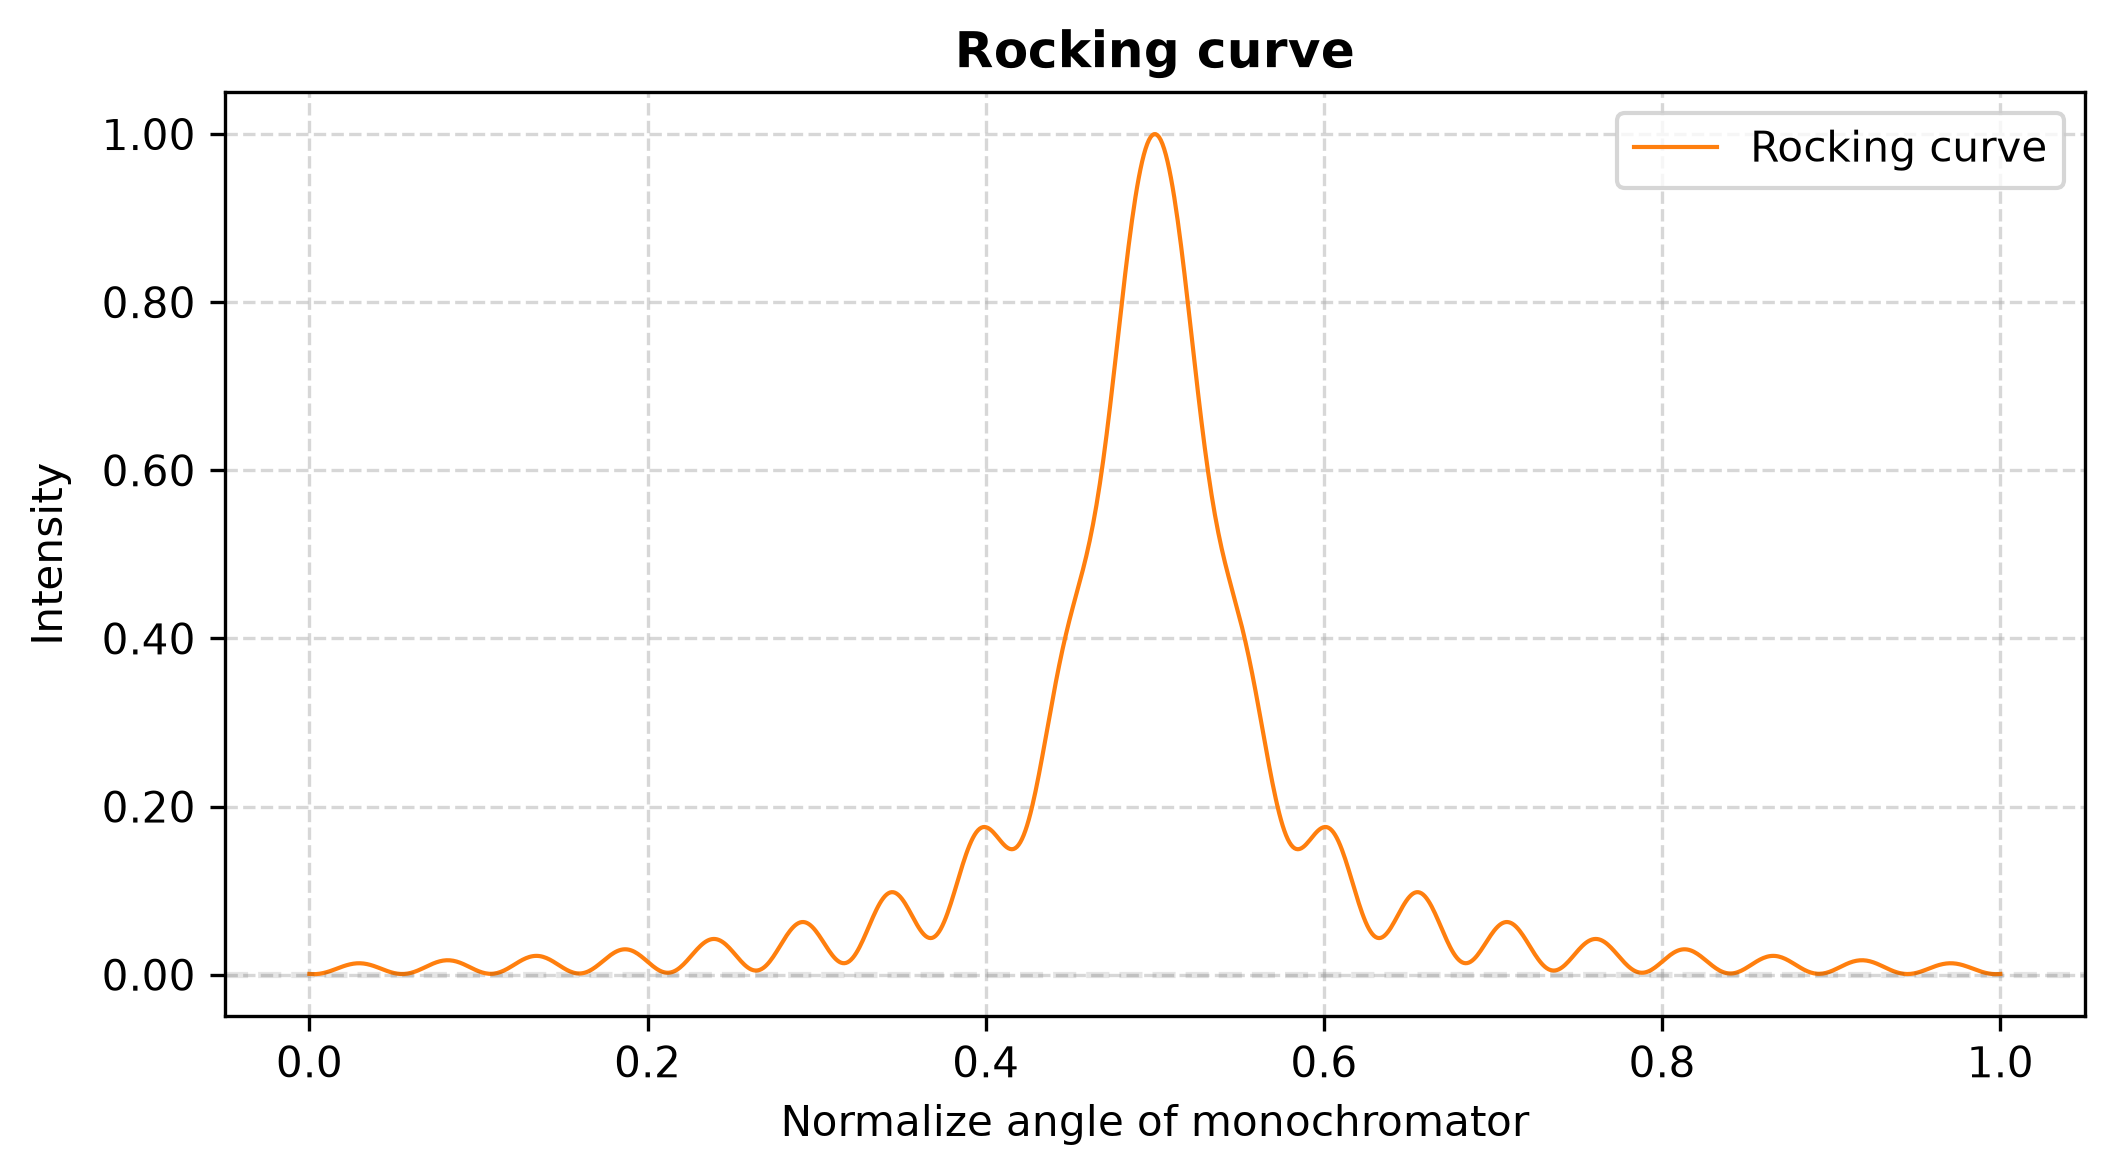
\includegraphics[width=0.85\textwidth]{img/cap 1/Rocking curve.png}
    \caption{Example of rocking curve with the angle of DCM normalize between 0 and 1, and the intensity peak normalize to 1}
    \label{fig:rocking curve}
\end{figure}

The largest peak in the graph corresponds to the angle that must exist between the two crystals to produce the maximum intensity.
The angle that produces the maximum beam intensity is not necessarily fixed, and if it were to move, it would cause the crystals to become misaligned.
Thermal variations, mechanical vibrations, and the hysteresis of piezoelectric actuators can alter the crystal alignment over time \cite{Proux2006,Stoupin2010}.

Peak intensity drift is a problem that cannot be solved by beam position control alone.
In fact, the position control system could maintain the correct location of the beam without ensuring the alignment of the monochromator, resulting in a degradation in intensity.
It is necessary to add a control system that takes care of tracking the intensity peak.

\section{Importance of Peak Intensity Tracking}

There are several reasons to operate at maximum beam intensity, some experiments actually require the highest available monochromatic photon flux. 
If the monochromator is not aligned correctly, some of the intensity will be lost before the beam reaching the sample.
Some experiments require counting photons until the required number is reached. 
If some photons are lost, the experiment will take longer to reach the required number of photons.

The stability of the system during experiments or beam scanning should not be underestimated.
Stability is also important during measurements that last several minutes or hours, or while the photon energy is scanned. 
If stability were to be lost, it would be difficult to compare experiments, which could change the interpretation of the data \cite{Proux2006,vanSilfhout2014,Quinn2021}.

The main goal of the thesis is to design a control system that not only finds the peak of intensity, but also follows it in case it moves.
This can be done by a feedback control loop which, based on the intensity produced, applies the right correction to change the angle between the two crystals of the monochromator in order to reach the peak intensity.

\section{Existing Beam Stabilization Solutions}

The problem of peak intensity oscillation has already been encountered and several solutions have emerged.
Some implemented solutions involve using position to change the intensity while others use components to directly change the intensity of the beam.
Changing the intensity directly via a monochromator is a non-trivial problem, since the intensity does not vary monotonically with the relative crystal angle.

Proux et al. \cite{Proux2006} describe their work done at the ESRF, specifically for a DCM cooled with liquid nitrogen.
The main idea of what they did is based on small adjustments using piezoelectric actuators and the use of lock-in to extract the gradient of the rocking curve.
The controller uses the gradient information to correct the angle between the monochromator crystals and keep it stable at the intensity peak.
The ESRF Monochromator Controller (MoCo) provides a related example of dedicated instrumentation \cite{MoCo2008}. 
MoCo provides three modes of operation: position, fixed intensity, and oscillation.
The latter injects a small disturbance to understand the gradient of the rocking curve through synchronous detection.

Stoupin et al. \cite{Stoupin2010} instead opted for another approach, namely the null-detection principle, for angular stabilization of optical components.
They were able to validate their proposal by testing with an angular stability of approximately $13\,\mathrm{nrad}$ RMS.
This demonstrates how sensitive the angle between the two crystals is and the usefulness of a control system even when the required corrections are very small.

Van Silfhout et al. \cite{vanSilfhout2014} proposed a system to simultaneously control both the intensity and the position of the beam.
To do this they used two independent systems, one for position and one for intensity.
This shows that the two problems, although dependent on each other, require distinct solutions, each with its own purpose.

Extremum-seeking, as mention before, can be used for beam stabilization too. 
In fact, Zohar et al. \cite{Zohar2016} used this approach to stabilize the beam intensity by introducing a small sinusoid to the piezoelectric
Although they did not directly modify the angle between the crystals of the monochromator, they managed to stabilize the intensity.
Their situation revolves around beam positioning through an aperture.
More recently, Quinn et al. \cite{Quinn2021} have implemented a combined control system at software level that allows both the position and the intensity of the beam to be managed simultaneously.

These work demonstrated the non-uniqueness of the solution for tracking the intensity peak.
The aim of this thesis is not to create a new solution, but based on what has already been done, implement it within the Beamline Enhanced Stabilization Technology (BEST) system \cite{BEST2024}.
With particular attention to the feedback control system and everything related to it.
The topics covered around the feedback control system will be: digital signal processing, controllers, delay introduced by the whole system (control, mechanism, actuator, etc...) and to the possible setting of parameters for different operating conditions.

\section{Feedback Control System}

The photon beam moves in time and for aiming it onto a target material, it requires a closed-loop feedback control system.
During the experiments the system must read the position of the beam from the beam and compute the correction needed for adjust the position of the photon beam.
The BEST system already has the position feedback control systems, but it cannot track the peak intensity of the photon beam.
The use of a feedback control approach has already been demonstrated, both for position control and for peak intensity tracking  \cite{Proux2006,MoCo2008,vanSilfhout2014,Quinn2021}.
Proportional-Integral-Derivative (PID) are controllers widely diffuse around different field and topics, from industrial to scientific domains. 
The key characteristics for his popularity are simplicity reliability and effectiveness.
A standard PID controller use the difference between the setpoint and the measured value for calculate the corrective control output and it is based on three distinct terms:

\begin{itemize}
    \item \textbf{Proportional (P):} Generates an output proportional to the current positioning error, scaled by a proportional gain factor.
    \item \textbf{Integral (I):} Accumulates past positioning errors over time to eliminate steady-state error and overcome system bias (with appropriate anti-windup mechanisms).
    \item \textbf{Derivative (D):} Evaluates the rate of change of the error signal to anticipate future trajectory shifts and damp transient responses.
\end{itemize}

The ideal continuous-time PID control function $u(t)$ can be expressed as:

\begin{equation}
    u(t) = K_p e(t) + K_i \int_{0}^{t} e(\tau) \, d\tau + K_d \frac{de(t)}{dt} 
\end{equation}

where $e(t)$ represents the positioning error, and $K_p$, $K_i$, and $K_d$ denote the proportional, integral, and derivative gains, respectively.

\section{Proposed Solution: Intensity Peak Tracking with the BEST system}


The thesis revolves around the integration of the peak intensity tracking system into the BEST system.
The system already created by ELS Instruments already has the position control system present but the peak tracking system discussed in this thesis is not present.
For reaching the goal of this thesis, it is needed to understand the Beamline Enhanced
Stabilization Technology (BEST) system first. 
It is then possible to achieve the goal, which is to add a peak intensity tracking system.

The BEST system architecture is composed by three main hardware modules: a \textit{TetrAMM}, a \textit{Central Unit} and a \textit{PreDAC}.

The primary control data flow operates as follows:
\begin{itemize}
    \item The \textit{TetrAMM} unit reads the photo-emitted currents from the beam position sensors, digitizes the signals, sends the 4 currents data to the \textit{Central Unit}.
    \item The \textit{Central Unit} converts the currents into positions and intensity, processes the feedback algorithm, calculate the necessary corrective displacements required to maintain target alignment and transmits control commands to the \textit{PreDAC}.
    \item The \textit{PreDAC} converts digital control commands from the The \textit{Central Unit} into high-precision analog voltage signals fed idrectly into the piezoelectric actuators.

\end{itemize}

\begin{figure}[htbp]
    \centering
    \begin{tikzpicture}[
        scale=0.85, transform shape,
        beam/.style={line width=1.5pt, orange!80!black},
        component/.style={draw, rectangle, rounded corners, thick, fill=blue!10, minimum width=2.2cm, minimum height=1.1cm, align=center, font=\small},
        bestblock/.style={draw, rectangle, dashed, thick, fill=red!5, minimum width=6.5cm, minimum height=2.0cm, align=center, font=\small},
        hardware/.style={draw, rectangle, thick, fill=gray!20, minimum width=2.4cm, minimum height=1.0cm, align=center, font=\small},
        cable/.style={thick, blue!50!black, -Stealth}
    ]

      % --- BEAMLINE LAYOUT ---
      \coordinate (source) at (0, {3.5 - 0.2*cos(10)});
      \coordinate (c1) at (3.2, 3.5);
      \coordinate (c2) at (5.8, 2.8);
      \coordinate (c3) at (5.8, 2.1);
      
      \coordinate (c1_bottom) at ($(c1) - ({0.2*sin(10)}, {0.2*cos(10)})$);
      \coordinate (c3_top) at ($(c3) + ({0.2*sin(28)}, {0.2*cos(28)})$);
      \coordinate (c2_bottom) at ($(c2) - ({0.2*sin(28)}, {0.2*cos(28)})$);

      \coordinate (det) at ($(c3_top) + ({2.2},{0})$);
      \coordinate (sample) at ($(det) + ({2.0},{0})$);

      % Draw X-ray beam path
      \draw[beam] (source) node[above, black, font=\bfseries] {Synchrotron Source} -- (c1_bottom);
      \draw[beam] (c1_bottom) -- node[above right, font=\footnotesize, black] {DCM} (c2_bottom);
      \draw[beam] (c2_bottom) -- (c3_top);
      \draw[beam] (c3_top) -- (det);
      \draw[beam] (det) -- (sample);

      % --- OPTICAL COMPONENTS (DCM & DETECTORS) ---
      \draw[thick, fill=cyan!30, rotate around={-10:(c1)}] ($(c1)+(-0.4,-0.2)$) rectangle ($(c1)+(0.4,0.2)$);
      \node[above=0.25cm, font=\small] at (c1) {Crystal 1 (Fixed)};

      \draw[thick, fill=cyan!30, rotate around={-28:(c2)}] ($(c2)+(-0.4,-0.2)$) rectangle ($(c2)+(0.4,0.2)$);

      \begin{scope}[shift={(c3)}, rotate=-28]
        \draw[thick, fill=cyan!30] (-0.4,-0.2) rectangle (0.4,0.2);
      \end{scope}

      % Ion Chamber / Detector (I0)
      \draw[draw, thick, fill=green!20] ($(det)+(-0.3,-0.6)$) rectangle ($(det)+(0.3,0.6)$);
      \node[above=0.6cm, font=\small, align=center] at (det) {BPM\\(Detector)};

      % Endstation / Sample
      \node[component] at (sample) {Sample /\\ Endstation};

      % --- ELS INSTRUMENTS BEST SYSTEM INTEGRATION ---
      \node[hardware] (predac) at (4.5, -0.6) {PreDAC\\(Actuator Module)};
      \node[hardware] (tetramm) at (8.2, -0.6) {TetrAMM\\(Readout Module)};

      \node[bestblock] (central) at (6.35, -4.0) {
        \textbf{ELS Instruments BEST Central Unit}
      };


      % --- CABLING & SIGNALS ---
      \draw[cable] (predac.north) -- node[right, font=\footnotesize] {Drive + Dither ($V$)} ($(c2)+(0,-0.8)$);
      \draw[cable] (det.south) -- node[right, font=\footnotesize] {Current Signals} (tetramm.north);
      \draw[cable, <->] (predac.south) -- node[left, font=\footnotesize] {Optical link} (predac.south |- central.north);
      \draw[cable, <->] (tetramm.south) -- node[right, font=\footnotesize] {Optical link} (tetramm.south |- central.north);

    \end{tikzpicture}
    \caption{Schematic layout of a synchrotron beamline optics and hardware integration using the BEST system. The X-ray beam reflects off the Double Crystal Monochromator (DCM), passes through the BPM for position and intensity readout, and reaches the endstation. Real-time position control loops executed on the Central Unit coordinate the PreDAC actuator module and TetrAMM readout module to keep position stable in a closed-loop fashion.}
    \label{fig:beamline_best_integration}
\end{figure}

The \textit{Central Unit} is composed by two main parts: a Field-Programmable Gate Array (FPGA), which is where run the real-time feedback control loop, and a industrial host PC.
The latter runs a custom graphical user interface (GUI) that allows you to view the beam position and modify the feedback control system.
The TetrAMM reads the currents produced by BPM and translates to digital signals and sends them to the Cental Unit.
The PreDAC on the other hand, reads the correction signal coming from the Central Unit and converts it into small analog voltage that move the actuators.
The three hardware modules are connected with a Small Form-Factor Pluggable (SFP) optical interfaces in order to have High-speed, low-latency and reduce noise pick-up inside the system.

The FPGA includes a soft-core processor that runs the control firmware, so the feedback loop can be executed at deterministic intervals while retaining the flexibility of a software-based control algorithm.

The method chosen for tracking the intensity peak is one of those mentioned above, which involves the insertion of a small dither signal, to the voltage that moves the piezoelectric actuator connected to the DCM.

Instead of calculating the intensity derivative from the raw noise data received from the TetrAMM, a pipeline consisting of digital filters and synchronous demodulation will be used.
First the intensity passes through a band-pass filter centered on the frequency of the dither signal.
Then the filtered signal is demodulated with a reference signal having the same frequency as the dither signal and finally it is filtered with a low-pass filter to obtain the intensity gradient, $\mathrm{d}I/\mathrm{d}\theta$.
Next, the gradient is sent to the PID, which will calculate the movement the actuator will have to make to reach the maximum intensity.

The time required to apply the dither signal and read its intensity response is considered delay time.
To this must be added the delay introduced by the filters.
This delay must be taken into account because demodulation is synchronous; otherwise, it would lead to incorrect demodulation, resulting in poor accuracy.
To overcome this problem, a routine for automatically calculating the phase delay has been included.
The routine includes in-phase, quadrature, and four-quadrant arctangent methods for calculating the phase delay.

Since the solution is composed of parameter-based methods, the ultimate goal is to make the parameters configurable.
The parameters in question are the amplitude and frequency of the dither signal, the filter coefficients, and the PID coefficients.
Starting from the parameterization made for the position control, it should be extended for the control on the intensity peak.
The design, implementation and validation will be explained in the next chapters.

\section{Thesis Outline}

The thesis is organized into five chapters. Chapter 2 reviews the feedback methods and signal-processing techniques used for beam stabilization and intensity tracking. Chapter 3 describes the proposed implementation within BEST, including the digital filtering pipeline, the PID control loop, and the automatic phase calibration procedure. Chapter 4 presents the validation of the system through simulation, together with the FPGA resource and timing checks and the analysis of the controller response. Finally, Chapter 5 discusses the conclusions of the work and the possible developments needed for testing the system on a physical beamline.

\newpage
\chapter{State of the Art and Literature Review}\label{chap:State of the Art and Literature Review}

\section{Introduction}

The result of an experiment that involves a synchrotron beamline depends on two factors: the beam itself and its stability.
The alignment of the photon flux can easily change due to different factors such as thermal deformation of optical components, mechanical drift.
This type of misalignment can cause a variation in the intensity of the beam and its position.
Some experiments have small apertures, heterogeneous samples, or energy-dependent measurements and in these cases these effects become more significant
\cite{Proux2006,vanSilfhout2014,Quinn2021,Zohar2016}.
The disturbance at the origin can be reduced by including improved mechanical design and thermal management.
Another solution for reducing the disturbance is to use an active feedback, it can adjust an optical component to compensate the drift during operations.
There are different kinds of possible experiments, usually the requirements are to control the beam position, to control the intensity of it, or a combination of both
\cite{Proux2006,vanSilfhout2014,Quinn2021}.
This chapter investigates how feedback methods were relevant to the development of a beam-control system for the peak intensity.
In the specific, the topics covered are monochromator rocking-curve optimization, modulation-based gradient estimation, software-based hill climbing, and the dependence between peak intensity tracking and the beam position stabilization.
The review is based on the systems found in Proux et al., Stoupin et al., van Silfhout et al., Zohar et al., and Quinn et al., end the ESRF MoCo documentation.
\cite{Proux2006,Stoupin2010,vanSilfhout2014,Zohar2016,Quinn2021,MoCo2008}.

\section{Definition of the Feedback Objective}

\subsection{Intensity maximization and intensity regulation}
First of all, it's necessary to distinguish between maintaining a target intensity and maintaining maximum intensity.
In the first case, the controller attempts to minimize an error of the form

\begin{equation}
    e_I(t)=I_{\mathrm{ref}}-I(t),
    \label{eq:intensity_setpoint_error}
\end{equation}

where $I_{\mathrm{ref}}$ is a specified intensity reference.
In the other case, no target intensity is set, since the controller must aim for the maximum of the intensity-response function.
\cite{MoCo2008,Quinn2021}.
For convenience, the term \emph{peak intensity} stands for the maximum of the intensity function.
Let $u$ represent an actuator command, it can be for example a voltage applied to a piezoelectric.
Let $I(u,t)$ represent the corresponding measured intensity. The peak-tracking objective is

\begin{equation}
    u^\star(t)
    =
    \operatorname*{arg\,max}_{u\in\mathcal{U}} I(u,t),
    \label{eq:peak_tracking_objective}
\end{equation}

where $\mathcal{U}$ is the admissible actuator range.
The time must be included due to interpolate the system drifts.
Instead of minimizing the error in the beam's position relative to the target.
The systems discussed here focus on the intensity transmitted or use a beam-monitor signal as an indirect measurement of the intensity.
\cite{Proux2006,Zohar2016,Quinn2021}.

\subsection{The monochromator rocking curve}

The type of monochromator discussed is the double-crystal, whose intensity depends on how the crystals are aligned with each other.
The relation between the intensity and angle is commonly described by a rocking curve.
The role of the feedback is to adjust the crystal's angle via the piezoelectric, in order to maintain the intensity at the maximum level.
\cite{Proux2006}.
Near a smooth local maximum, a useful analytical approximation is the second-order Taylor series expansion

\begin{equation}
    I(u,t)
    \simeq
    I_{\max}(t)
    -
    \frac{c(t)}{2}
    \left[u-u^\star(t)\right]^2,
    \qquad c(t)>0.
    \label{eq:local_peak_model}
\end{equation}

It is not necessarily the case that rocking curves have a globally parabolic shape, this expression can be used to approximate a local portion of it and this is used to explain the feedback principle.
The derivative of the approximation is

\begin{equation}
    \frac{\partial I}{\partial u}
    \simeq
    -c(t)\left[u-u^\star(t)\right].
    \label{eq:local_peak_gradient}
\end{equation}

By looking at the sign of the derivative it is possible to know in which direction to make the correction.
At the maximum, the gradient is zero.
To try to achieve maximum transmission, seeking a zero gradient alone is not sufficient, minima and flat regions have small derivatives too.
Tracking peak intensity needs an appropriate acquisition or tuning procedure, an appropriate operating
range, and sufficient signal sensitivity.
MoCo provides functions for automatic tuning and shows how tuning can be impactful even before regulation begins 
\cite{MoCo2008}.

\section{Modulation-Based Peak Tracking}

\subsection{Gradient estimation by synchronous detection}

A common method is to introduce a tiny sinusoidal noise and measure the corresponding intensity response. 
With this approach, it is possible to understand the direction of the adjustment, which is absent from a single intensity measurement
\cite{Proux2006,Stoupin2010,Zohar2016}.
For example, if we consider a command 

\begin{equation}
    u(t)=\bar{u}(t)+a\sin(\omega_m t),
    \label{eq:dither_input}
\end{equation}

where $\bar{u}$ is the slowly varying operating point, $a$ is the modulation amplitude, and $\omega_m$ is the modulation angular frequency. 
With a small modulation, the response is approximately static over one period

\begin{equation}
    I(u(t))
    \simeq
    I(\bar{u})
    +
    a I'(\bar{u})\sin(\omega_m t)
    +
    \frac{a^2}{2}I''(\bar{u})\sin^2(\omega_m t).
    \label{eq:dither_expansion}
\end{equation}

If the equation is multiplied by a phase-aligned sinusoid and followed by low-pass filtering, it gives

\begin{equation}
    g(t)
    =
    \operatorname{LPF}
    \left\{
        I(t)\sin(\omega_m t)
    \right\}
    \simeq
    \frac{a}{2}I'(\bar{u}).
    \label{eq:demodulated_gradient}
\end{equation}

The numerical scaling of the $g(t)$ depends on three factors: reference waveform, normalization and implementation.
Under the idealized sign convention of
Equation~\eqref{eq:demodulated_gradient}, a gradient-ascent law is

\begin{equation}
    \frac{d\bar{u}}{dt}=k g(t),
    \qquad k>0.
    \label{eq:ideal_gradient_ascent}
\end{equation}

Combining this law with Equation~\eqref{eq:local_peak_gradient}, it is possible to acknowledge the local convergence toward the maximum in a simplified quasi-static scenario.
Theory and practical implementation differ by some key aspects like actuator polarity, phase lag, detector response, filtering and control delay.
As has been observed by Zohar et al., these dynamics influence convergence and residual oscillations \cite{Zohar2016}.

\subsection{Spatial or actuator gradients versus time derivatives}

For tracking the intensity peak it is necessary to track its own derivative with respect to the controlled optical coordinate.
Generally the time derivative is not equivalent in this case, because following the next equation 

\begin{equation}
    \frac{dI}{dt}
    =
    \frac{\partial I}{\partial u}\frac{du}{dt}
    +
    \frac{\partial I}{\partial t}.
    \label{eq:temporal_vs_actuator_derivative}
\end{equation}

The equation shows that there is a term that doesn't change with the commanded actuator motion.
It follows that, if the intensity decreases, it's not possible to know the direction in which the actuator should move.
Knowing the reference signal used in synchronous detection allow to extract the intensity variation correlated with optical motion.

\section{Early Demonstrations and Precision Stabilization}

\subsection{Proux et al.: feedback for a cryogenic monochromator}

Proux et al. proposed an active alignment feedback for double-crystal monochromator cooled with nitrogen liquid \cite{Proux2006}. 
Their solution spans both thermal and mechanical aspects with ensuring optimal transmission during beamline operation.
Piezoelectric was used as actuator for adjust the relative angle of the crystal by the feedback.
This controller is suited to operate at the top of the rocking curve instead of working on a selected target on one of its slopes.
The advantage of working on top of the curve is that the alignment condition is identified by a derivative-zero criterion instead of a fixed absolute intensity. 
If the flux changes, the criterion doesn't, because the zero of the derivative stays the same when it acts as a multiplicative scaling.
This can be practically useful if the source is changed or during energy scans
\cite{Proux2006}.
The derivative zero invariance is different from the invariance of all closed-loop dynamics.
When working with the local model, if the intensity is multiplied by a positive factor, it also influences the estimated gradient.
In this manner it also changes the effective loop gain, thus a compensation is needed.
During robustness assessment, it is necessary to differentiate the location of the optimum and the dynamics of the convergence.

\subsection{Stoupin et al.: nanoradian angular stabilization}

Stoupin et al. used a null-detection feedback system for investigating angular stabilization \cite{Stoupin2010}. 
His experiments have been conducted with a high-energy-resolution monochromator and a high-set-load monochromator due to the stringent alignment requirements.
Angular stability was demonstrated $13\,\mathrm{nrad}$ RMS approximately \cite{Stoupin2010}.
The work done doesn't stop at maximizing transmitted flux.
It also shows that the intensity derivative can be used for the understanding of align reference.
In this way a communication bridge is created between peak-seeking feedback and the high-resolution angular stabilization.
Although they are dependent, the angular stability must be distinguished from intensity stability.
It is possible to derive one quantity from the other, but one must take into account the presence of local rocking curve shape, operating point and other sources of photon flux. 
That being said, from a nanoradian angle it's impossible to know the relative intensity stability without additional information.

\section{ESRF MoCo}

\subsection{Controller architecture and operating modes}

The ESRF Monochromator Controller, MoCo, is a custom electronic module for regulating an optical component using as input a beam-monitor signal. 
The inputs and outputs of this system are: an incoming-beam signal, INBEAM, an outgoing-beam signal, OUTBEAM and a voltage output connected to an optical actuator \cite{MoCo2008}.
The manual distinguishes three closed-loop modes:

\begin{enumerate}
    \item \emph{Position mode}, in which a beam-position signal is regulated to a fixed reference.
    \item \emph{Intensity mode}, in which operation is maintained
    at a selected relative intensity on either side of a
    transmission peak.
    \item \emph{Oscillation mode}, in which a small modulation
    is added to the drive and synchronous detection produces
    a derivative-related feedback signal.
\end{enumerate}

Only the third mode provides continuous peak regulation using
a derivative-zero condition \cite{MoCo2008}.

\subsection{Control and operational functionality}

MoCo's PID is limited to the integral correction rather than having a complete PID.
The feedback system must be regulated based on the response of the optical system (actuator, mechanics, detector).
Other than the feedback, the controller takes care of incoming-beam normalization, automatic tuning, beam-presence detection, pause and inhibit functions and an interlock interface.
MoCo has two types of synchronous measurements, main and quadrature, they both allow the detection phase to be adjusted \cite{MoCo2008}.
All of these properties establish that the controller is more than a peak-search algorithm.
In fact, the controller has to distinguish misalignment from beam loss, do not make trivial corrections during interruptions, and resume operation in a controlled manner.

\section{Combined Intensity and Position Stabilization}

\subsection{Van Silfhout et al.: separate observables and feedback loops}

Van Silfhout et al. achieved stabilization of photon flux and beam position using two independent feedback loops based on different inputs (flux and position measurements).
The authors tested this approach with EXAFS scans at the titanium K-edge \cite{vanSilfhout2014}. 
Maximizing photon throughput is achieved with a fast algorithm extremum-searching, which is insensitive to changes in storage-ring current and energy-dependent monochromator output.
Instead, for correcting the position use the signals emitted by beam-position monitor.
The validity of the method is evaluated on an experiments, which involve measurements of inhomogeneous and diluted titanium-containing samples with and without feedback \cite{vanSilfhout2014}.
The authos emphasize and demonstrate why flux optimization and position stabilization should treated differently. 
The flux optimization controller may adjust the the monochromator's transmission, with the goal of hit the peak of the intensity while changing the position of the beam.
In the same way the the position stabilization controller may get in the way of the other controller.
As already noted, some experiments need to, both position and intensity fixed.
For example, when dealing with heterogeneous samples, the beam motion can change the material volume being probed, thus modify the recorded spectrum \cite{vanSilfhout2014}.

\subsection{Zohar et al.: alignment through transmitted-intensity optimization}

Zohar et al. extend extremum-seeking feedback to vertical beam-position stabilization at a small aperture \cite{Zohar2016}. 
The system exploits the aperture for maximize the intensity through mirror instead of directly regulating a position measurement. 
The controller reuses the beam oscillations already present due to intensity feedback.
Knowing the phase reference supplies information about the spatial intensity gradient while reading intensity downstream.
No additional perturbation is introduced specifically for the position-control loop \cite{Zohar2016}.
Tests were made for testing the proposed solution, the first was introducing a misalignment and in less than $6\,\mathrm{s}$.
The second test was for the intensity stability, the result was  $1.5\%$ FWHM (Full Width at Half Maximum) through a $5\,\mu\mathrm{m}$ aperture over an eight-hour measurement.
The authors also observe the existence of a trade-off: achieving faster convergence can lead to larger residual actuator oscillations \cite{Zohar2016}.
The reported $1.5\%$ value is a FWHM measure, not an RMS value.
This decision was made due to the nature of the distribution, which isn't symmetric.
Thus, converting FWHM to RMS for using Gaussian distribution need additional justification \cite{Zohar2016}.
This proposed approach shows that the optimized signal changes physical meaning based on the location of the detector.
If the detector is immediately placed after a monochromator, it primarily measures its transmission. Meanwhile, if the detector is placed after a restrictive aperture, it measures the quality of the beam.

\section{Software-Based Peak Tracking}

Quinn et al. propose a software-based feedback system on the I14 hard X-ray nanoprobe beamline at Diamond Light Source \cite{Quinn2021}.
The system is composed of two parts, the first one tries to maximize the intensity through monochromator adjustment. The second part is a PID that controls the position of the beam through a mirror.
The reasoning that led to this solution was a direct consequence of the practical limitations associated with transferring hardware-specific feedback systems between beamlines that employ different control architectures.
This leads to an alternative solution, using a software implementation; in this way is possible to integrate the feedback with existing beamline infrastructure \cite{Quinn2021}.
To optimize the intensity, we scan the second monochromator crystal through EPICS, covering roughly $\pm100\,\mathrm{nrad}$ in $25\,\mathrm{nrad}$ steps at $5\,\mathrm{Hz}$. 
Once the maximum is found by a hill-climbing routine, the centre of the next sweep is shifted onto it \cite{Quinn2021}.
This method can result similar to lock-in detection, but the way the directional information is obtained is different.
While lock-in methods use a periodic excitation to estimate a gradient, the software hill-climbing uses discrete intensity comparisons.
As was already stated, the monochromator adjustment affects both intensity and position of the beam, the problems aren't independent.
Between successive intensity-search steps, the position loop is updated.
Alternating optimization makes sure to address the interaction between the controllers without assuming that the loops are physically decoupled \cite{Quinn2021}.
The author decided to use fixed update rate of $5\,\mathrm{Hz}$ that isn't related to the closed-loop bandwidth.
Nonetheless, the convergence depends on the search sequence, measurement response, and disturbance magnitude.
If large energy change is detected, the implementation breaks down into intermediate steps allowing settling time \cite{Quinn2021}.
Quinn et al. tell to use the system for two years and as possible future development to switch on Kalmanfilter for the estimation.
These extensions can't be proposed as solution as they weren't implemented or tested \cite{Quinn2021}.

\section{Literature Comparative Assessment}

The table~\ref{tab:sota_comparison} summarizes all the systems mentioned above and cites their individual contributions.
The studies have different backgrounds, thus instead of comparing them by their performance, they are compare based on their implementation principle and objective. 

\begin{table}[htbp]
    \centering
    \small
    \caption{Comparison of the feedback approaches reviewed in this chapter.}
    \label{tab:sota_comparison}
    \begin{tabularx}{\textwidth}{@{}p{0.19\textwidth}XX@{}}
        \toprule
        Reference & Main objective & Distinctive contribution \\
        \midrule
        Proux et al.\ \cite{Proux2006}
        & Maximum monochromator transmission
        & Lock-in-based alignment feedback integrated with
          a cryogenic monochromator. \\
        Stoupin et al.\ \cite{Stoupin2010}
        & Precision angular stabilization
        & Null-detection feedback with demonstrated
          nanoradian-scale angular stability. \\
        MoCo manual \cite{MoCo2008}
        & Position, relative intensity, or peak tracking
        & Dedicated controller with distinct operating modes
          and operational supervision. \\
        van Silfhout et al.\ \cite{vanSilfhout2014}
        & Simultaneous flux and position stabilization
        & Separate measurements and independent loops,
          validated using EXAFS measurements. \\
        Zohar et al.\ \cite{Zohar2016}
        & Beam alignment at an aperture
        & Spatial-gradient estimation using an existing
          beam oscillation. \\
        Quinn et al.\ \cite{Quinn2021}
        & Intensity and position control during energy changes
        & Software hill climbing interlaced with position PID. \\
        \bottomrule
    \end{tabularx}
\end{table}

\subsection{Gradient quality and disturbance rejection}

For an explanatory measurement model

\begin{equation}
    I_{\mathrm{meas}}(u,t)
    =
    A(t)F(u,t)+b(t)+n(t),
    \label{eq:intensity_measurement_model}
\end{equation}

where $A(t)$ is multiplicative source or gain variation, $F(u,t)$ is the optical transmission response, $b(t)$ is an additive background and $n(t)$ is noise.
If $A(t)$ is positive and doesn't depend of $u$, it means the location of the maximum of $F$ doesn't change.
Still, it can interfere with intensity comparisons if switched to a discrete search, this can happen because when $A(t)$ change its magnitude can alter the effective gain of derivative-based feedback.
This emphasizes why such practice like source normalization and robustness to changing flux are important during implementation \cite{MoCo2008,vanSilfhout2014}.
During the phase of synchronous detection, contributions that are not correlated with the reference after averaging are suppressed. 
However some disturbances can still pass.
If the disturbances pass near the modulation frequency or phase error, it may end up affect the estimated gradient.
MoCo shows how the main and quadrature influence the phase and their relationship to it \cite{MoCo2008}.

\subsection{Perturbation amplitude and measurement impact}

The modulation is constrained by a trade-off, it has to be large enough to generate a measurable response and in the same time small enough to avoid disturbance.
The local expansion described from Equation~\eqref{eq:dither_expansion}, the average intensity is approximately

\begin{equation}
    \langle I\rangle
    \simeq
    I(\bar{u})
    +
    \frac{a^2}{4}I''(\bar{u}).
    \label{eq:mean_modulated_intensity}
\end{equation}

Operating at the peak intensity, the injected modulation makes drop the average intensity by a square factor of the modulation amplitude $a^2$.
The modulation put into the monochromator not only alters the intensity value, but also causes a change in the position of the beam.
Different approaches were taken by the authors: Zohar et al. exploit this coupling, whereas Quinn et al. emphasize keeping the perturbation sufficiently small for nanoprobe measurements \cite{Zohar2016,Quinn2021}.

\section{Summary}

The literature mentioned before proposed two main methods for tracking intensity peak: modulation-based derivative estimation with null regulation, and discrete perturb-and-observe searches.
The first solution was designed by monochromator feedback and dedicated controllers such as MoCo.
While the second was proposed by Quinn et al. with a software implementation 
\cite{Proux2006,Stoupin2010,MoCo2008,Quinn2021}.
There are some details you need to pay attention to, maximizing monochromator transmission can destabilize the beam at the sample.
Based on the optical layout and experimental objective may require a separate position feedback or intensity measurements downstream of an aperture \cite{vanSilfhout2014,Zohar2016,Quinn2021}.
A possible solution must take into account measured observable, gradient estimator, feedback dynamics, actuator and supervisory functions.
All these factors are connected to each other and must be applied to the specific hardware and must be evaluated in the next chapters.
\chapter{System Architecture and Implementation}\label{chap:System Architecture and Implementation}

As mentioned before, the solution proposed in this thesis is an addition on what is already done by ELS Instruments. 
The company already makes available the position control, therefore the architecture is already designed and implemented.
What is missing, is the adjustment for the case of peak tracking control.
The architecture of the BEST is heterogeneous, and involve the knowledge of different programming languages, even for implementing another type of control such as peak tracking control.
For implementing the solution of this thesis, it was necessary to get hands-on with various parts of the BEST system's software.
Starting with Quartus II for configure the logic of the FPGA, which in this case was necessary for outputting the value of the intensity derivative.
Quartus II is a powerful tool capable of many actions, for example design the logic of the FPGA.
But it's possible to synthesize custom blocks for doing the needed functions, for example write the intensity derivative value in a shared memory.
The shared memory can be read from programs through the BEST library, which is a library wrote for interface with the driver of the FPGA.
Inside Quartus II it's possible to code the program that will run inside the soft-core, in this specific case the soft-core was Nios II. 
Quartus II provides the IDE Eclipse for Nios II and the language used was C, this part was done for calculating the derivative and implementing the controller for the intensity tracking.
The last main part of the project was the local GUI, which is necessary for having a feedback on what the FPGA is doing by a Graphical User Interface (GUI).
The GUI wasn't used only for monitoring the FPGA but for configure some parameters of the FPGA, too. 
The development environment in this case is Qt Creator which is framework based on C++.
These were the three main components that needed changes for implementing the solution proposed by this thesis. 
The controller logic itself is described into a dedicated sub-section.

\begin{figure}[htbp]
    \centering
    \begin{tikzpicture}
    \end{tikzpicture}
    \caption{Lo schema inziale di Paolo magari semplificato}
    \label{fig:hw_sw_architecture}
\end{figure}


\section{FPGA System Integration and Qsys Interconnects}
\label{subsec:fpga_qsys_integration}

The foundational architecture provided by ELS Instruments is based on a compiled FPGA bitstream optimized for position the beam at the target position. 
To add another type of controller like peak tracking, the FPGA must be recompiled for accommodate the new block that will expose the first derivative and the new connections for connecting the new block with the already existing ones.
These modifications were done inside an Intel Quartus II's tool, Platform Designer (Qsys).
Qsys is a graphical interface that allow to build, configure and connect digital hardware systems using intellectual property (IP) cores, processors, memories, and peripherals.
Furthermore inside Qsys, is possible to import verilog files to synthesize new type of intellectual properties.
Once added, the IP rights must be configured by specifying the role of each input and output pin.

\subsection{Modification of the Qsys System Project}

The entry point of the project that encloses it, is a Qsys file; it instantiates the processors, peripherals, communications controllers and custom hardware accelerators.
For adding the solution proposed by this thesis is required to alter the topology of the project by adding connections and a block:
\begin{itemize}
    \item \textbf{Custom IP:} it was the block capable of receiving the first derivative of the intensity calculate the soft-core, it was added inside the subsystem that contain the soft-core responsible for position control and future peak intensity tracking.
    \item \textbf{Clock Domain and Reset Alignment:} The custom block was synchronized to the system clock domain, so that it is compliant with the rest of the system.
    \item \textbf{Export connection:} Because the Custom IP was inside a subsystem, for adding the derivative to the shared memory it need to be export outside of the subsystem.
    \item \textbf{PreDMA connection:} This connection link the subsystem that deals with signal processing with the Direct Memory Access which is the shared memory
\end{itemize}

This what was need to modify for exporting the derivative outside of the FPGA. More details on how the shared memory work is described in a subsection below.

\subsection{Avalon Interface Bus Architecture}
The communication between the block inside the FPGA are based through a system-level interconnect fabric, which in this case is the Avalon Interconnect Fabric.
Unlike the traditional shared system bus where only one device can talk, the Avalon Interconnect Fabric uses a slave-side arbitration and switch-fabric architecture.
These type of protocols allows multiple master to communicate to multiple slave simultaneously provided that the data exchange does not involve the same sources or destinations.
Avalon provide three main type of standardize interface for the communication between the blocks, although is possible to create a custom communication instruction.
\begin{itemize}
    \item \textbf{Avalon Streaming (Avalon-ST) for Data Paths:} Used for high-speed, unidirectional, point-to-point data streams (e.g., reading the TetrAMM output and passing it to another block). It bypasses address decoding to achieve high bandwidth with minimal latency.
    \item \textbf{Avalon Memory-Mapped (Avalon-MM) for Control and Telemetry:} The soft-cores reads or writes data by executing standard load/store assembly instructions targeting a specific addresses. Every block is assigned a unique address range. 
    \item \textbf{Avalon Conduit for Signal routing:} Used for send signals outside of the Avalon Interconnect Fabric to the physical pins of the FPGA.
\end{itemize}

\section{Shared Memory and DMA Data Transfer}

Although the FPGA can handle a fast flow of data, to communicate it to the host PC without affecting performance it is necessary to use an adequate solution.
The DMA allows devices to transfer data directly to and from system memory, freeing the CPU from the operation.
This way the host PC can query the FPGA via drivers to read data that is already present in the shared memory without having to slow down the FPGA itself.

\subsection{On-Chip Shared Memory Architecture}
The data stored in the shared memory ranges from raw data such as beam position to control system variables such as PID coefficients. 
Other variables, such as the first derivative of intensity and other parameters for solution simulation, have also been added.
Dealing with a continuous stream of data that is faster than the calls one can make to read that data, it is necessary to take a few precautions:
\begin{itemize}
    \item \textbf{Dual-Port RAM Blocks:} The shared memory is configured in a way that is accessible by the soft-core processor and the block that handles data delivery to the host PC.
    \item \textbf{Circular Buffer Implementation:} Instead of having a dynamic memory allocation, a circular buffer was implemented. In this way the memory has always the latest updated data. So, to function, the firmware always overwrites the oldest data.
\end{itemize}

\subsection{Direct Memory Access (DMA) Offloading}

To read telemetry data without blocking the soft-core that handles the control system:
\begin{itemize}
    \item \textbf{Hardware-Assisted Transfers:} An Avalon-ST/MM DMA controller was integrated into the system topology to handle bulk data transfers independently of the Nios II CPU.
    \item \textbf{Minimizing CPU Interrupt Overhead:} By utilizing DMA, the softcore processor is freed from executing explicit byte-by-byte copy routines. Instead, the DMA controller signals the CPU only upon completion of a block transfer, ensuring that deterministic execution bounds for the extremum-seeking control loop remain strictly uncompromised.
\end{itemize}

\section{Driver and BAR (Base Address Register)}

To allow the PC host to communicate with the FPGA hardware peripherals for setting parameter or already mention before for reading the data, it was established a device driver.
The driver use designed to match the corresponding operating system that in this case was Linux. 

\subsection{PCIe Bus Enumeration and BAR Mapping}
The host PC communicates with the FPGA via a PCIe connection, it knows the addresses thanks to the base address register (BAR).
The BARs tells to the system how much continuous memory the device need and what type of space it is.
During system boot phase and device enumeration:
\begin{itemize}
    \item \textbf{Base Address Register (BAR) Configuration:} The system allocates physical memory windows via the PCIe Base Address Registers. These BARs map the FPGA's internal memory-mapped control registers, status flags, and shared DMA buffers directly into the host system's physical address space.
    \item \textbf{Memory-Mapped I/O (MMIO):} By utilizing these mapped regions, software layers can read or write to hardware registers (such as dither parameters, filter coefficients, and status flags) with minimal access latency, avoiding the overhead of complex packet-based network stacks for local register tuning.
\end{itemize}

\subsection{Character Device Driver Modifications}
For exposing the shared memory containing the measurement made by the BPM and the additional values of the control system inside the FPGA to the host:
\begin{itemize}
    \item \textbf{Kernel-to-User Space Bridging:} The existing device driver architecture was inspected and understood for tracking down the paths made by the data to reach the host. The idea was to use the data channel already employed to pass further data such as the first derivative. 
    \item \textbf{Data Interception and Tracing:} The driver serves as an intermediate software to allow the host to communicate with the FPGA and vice versa. Thus, the job done by the driver is to prepare the data from the FPGA and make them presentable to the host, which can then be displayed on the screen using the local GUI.
\end{itemize}

\section{Nios II Softcore Subsystem and Eclipse Firmware Development}

Writing firmware inside a FPGA requires hardware-software co-design flow, Platform Designer, and the Nios II Software Build Tools (SBT) for Eclipse.
Once the hardware design is programmed into the FPGA (using Platform Designer), software development moves to the Nios II SBT for Eclipse.
The firmware run on a Nios II soft-core processor.
The main idea of soft-cores are they can handle Complex state machines, protocols, control flows and it is easier to write and maintain in a high-level software language like C.
The controller software was implemented by following the interrupt service routine (ISR).
Every time the soft-core receive a specific interrupt event, it trigger the position control feedback.
Thus, instead of doing the position control there is an option to use the lock-in system for intensity peak tracking.
It also outputs a byte stream representing the value of the first derivative.

\section{Supervisory Qt (C++) Desktop Interface and Parameter Tuning}
Qt Creator is a cross-platform Integrated Development Environment (IDE), it support multiple languages and in this case was adopted C++.
The developed program was created for multiple purpose, for having a visual feedback of the controller and the beam like position and intensity. 
And to manage or to configure the parameters of the controller if needed.
The program which use a graphical user interface (GUI), is unable to can dialogue directly with the FPGA.
the GUI must interface with the library in order to communicate with the FPGA.
\begin{itemize}
    \item \textbf{Parameter Injection:} Operators can dynamically adjust control loop configuration parameters—such as which channel represents what, PID parameters and other parameters for lock-in that allow for its flexibility. The Qt application serializes these commands and use the library for configuring the controller.
    \item \textbf{Real-Time Telemetry Visualization:} The modified Qt libraries read and process the DMA. It display the basic values such as the current of the BPM, the position of the beam or its intensity, the output of the DAC and the first intensity derivative.  
\end{itemize}

\section{Lock-in}

The Lock-in is a type of amplifier, which can extract a signal when the measurement is affected by noise.
Separating the signal of interest from the noise can only be done by knowing its frequency.
The main concept involves the use of a reference signal with known frequency and phase to extract the signal of interest.
This operation is called phase-sensitive detection.
For the realization of this thesis, the lock-in technique was used to calculate the first derivative of the intensity with respect to the monochromator angle.
in this case the sinusoidal signal to be extracted is inserted into the piezoelectric actuator and it is called dither signal.
As the actuator moves, it will move the DCM crystal, which in turn will cause an oscillation in the intensity measured by the BPM.
Since the dither signal is an artificial signal that will be added by the control system, its frequency is known, so it is possible to use a reference signal with the lock-in technique to extract the intensity variation caused by the dither signal.
Therefore, the intensity variation caused by the dithering signal can be extracted from the other components of the dithering signal.
The lock-in amplifier described in this thesis was built entirely in digital format.
Going into detail, the signal is first filtered through a band-pass filter centered on the dither signal frequency.
Filtering is done to remove unwanted components and remove noise.
The next step after filtering is to modify the intensity signal with the reference signal's sine wave, which has the same frequency as the dither signal. 
This results in a signal composed of two components: the first is DC, while the second component is at twice the frequency of the dither signal.
Since the zero-frequency component corresponds proportionally to the amplitude of the intensity oscillation, to isolate it from the other component it is necessary to filter it with a low-pass filter.
The reference signal to function correctly also requires the phase difference between the reference signal and the dither signal. 
The phase difference is contributed by several factors such as the electronics or mechanical components of the system which impact the demodulation.
Since the phase difference is a component to be taken into account, it must be calculated to correctly align the reference signal with the measured response.
So if the phase has been calculated correctly and the amplitude of the dither signal is small enough, the result obtained is proportional to the first derivative of the intensity with respect to the monochromator angle.
In this way the PID controller, based on the derivative, determines in which direction to turn the crystal to orient it on the intensity peak.
The implementation and details of the methods used to implement lock-in will be explained in the next section.


\section{Closed-loop feedback}

The solution's keys components are the Taylor expansion series, the Lock-in Amplifier and the PID already mention before.
Considering a function $f(x)=I$, where x represent the angle of the crystal and I the intensity produced by the beam position monitor.
From a fixed angle $\theta_0$ and for small changing in x it is possible to use Taylor expansion of $f(x)$ to the first order

\begin{equation}
    put-formula-of-taylor-expansion
\end{equation}


where $f'(x)$ depend on the small movement $\Delta\theta$.
In this case the small movement is set artificially, a small noise is injected into the movement of the piezoelectric.
The noise in this case is called reference signal and it is a sinusoidal function with a know frequency $w_{r}$ and amplitude $\alpha_r$.
And combined with the actual position of the monochromator, the equation result in:

\begin{equation}
    equation-of-theta
\end{equation}

The first component is also time-dependent, as it can be influenced by mechanical friction, piezoelectric hysteresis, etc.
The second key aspect of the solution is the lock-in amplifier, it is a method used for recover small signal in presence of overwhelming noise environment.
Thus it possible to recover the effect of the reference signal on the intensity of the beam.
Once the signal is recovered, it will then be passed to the PID which will calculate the movement that the monochromator will have to make to reach the peak.
Starting from the rocking curve graph, we can notice that to the left of the peak the derivative is less than zero while to the right it is positive.
Then setting the PID setpoint to zero, it can manipulate the position of the monochromator so as to set it to the peak intensity.
In this way it is not necessary to know the value of intensity peak for the PID to work.

\subsection{Principle of Phase-Sensitive Demodulation}
Starting from the equation of the monochromator's angle, it is possible to expand the measure intensity $I(\theta)$ via a Taylor series around the operating point $\theta_0$:

\begin{equation}
    I(t) \approx I(\theta_0) + \left.\frac{dI}{d\theta}\right|_{\theta_0} a \sin(\omega_d t) + \frac{1}{2}\left.\frac{d^2I}{d\theta^2}\right|_{\theta_0} a^2 \sin^2(\omega_d t) + \dots
\end{equation}

The derivative of the first order contains the directional gradient component modulated at the fundamental reference signal frequency $\omega_r$. 

\subsection{Demodulation and Filtering Pipeline}
Starting from the noise signal received by the BPM, it is need to isolate the gradient component $\left.\frac{dI}{d\theta}\right|_{\theta_0}$.
Digital lock-in tools allow the incoming signal to be processed to filter out all non-gradient components through a sequential four stage pipeline:

\begin{enumerate}
    \item \textbf{Band-Pass Filtering (Dither Pre-Selection):} 
    Before starting demodulate the raw intensity signal, it is filter with a pass-band filter center at the dither frequency.
    In this way is possible to remove the DC offsets, low-frequency drift and the analog for the high frequencies.
    This filter phase ensure only signal components around the dither frequency enter the mixer.
    
    \item \textbf{Mixer Stage (Multiplication):} The filtered intensity signal $I(t)$ is multiplied by the dither signal without amplitude and shifted by a phase delay introduced by the system itself:
    \begin{equation}
        M(t) = I(t) \cdot \sin(\omega_d t + \phi)
    \end{equation}
    This multiplication takes the gradient amplitude to the DC offset ($0\text{ Hz}$) and all the carrier noise is shifted on higher frequency along with the high-order harmonics.

    \item \textbf{Low-Pass Filtering (Integrator Stage):} 
    After mixing then signal is then filtered with a low-pass filter for removing all the noise and high-order harmonic.
    The remain component of the mixed signal is the DC output voltage $V_{demod}$ which is directly proportional to the current slope of the rocking curve:
    \begin{equation}
        V_{demod} \propto \left.\frac{dI}{d\theta}\right|_{\theta_0} \cos(\phi)
    \end{equation}

    \item \textbf{PID Feedback and Piezo Actuation:} The signal once demodulated, is taken as input for the PID controller which job is to drive the PreDAC piezoelectric actuator:
    \begin{equation}
    u(t) = K_p V_{\mathrm{demod}}(t) + K_i \int_0^t V_{\mathrm{demod}}(\tau) \, d\tau + K_d \frac{dV_{\mathrm{demod}}(t)}{dt}
    \end{equation}
    When the system reaches peak intensity, the slope becomes zero; this forces the controller to keep the voltage applied to the piezoelectric device constant, thereby ensuring that the monochromator is positioned to achieve maximum beam intensity.
\end{enumerate}

\subsection{Phase Alignment}
A practical issue with this technique is the time delay introduced by the physical system; this creates a desynchronization between the dither signal applied to the piezo and the reference signal used for mixing with the intensity signal.
If the delay is not considered, the gradient error is calculated by $\cos(\phi)$. 
Therefore, to avoid misalignments, it is necessary to include a controller startup phase during which the phase delay is calculated.

\paragraph{Calibration Algorithm and Execution Flow:}
The startup phase is based on the following sequence:
\begin{enumerate}
    \item \textbf{Operating Point Initialization:} The system drive the DMC across its range to have the rocking curve.
    From the rocking curve is possible to know where the peak intensity is and consequently establish a point at which to begin the calibration phase (e.g., at the half-maximum point of the rocking curve slope where the gradient is steepest).
    \item \textbf{Dynamic Warm-up and Excitation:} The dither signal is inserted into a predetermined time window. This sampling phase is used to acquire the data needed to calculate the phase delay.
    \item \textbf{Quadrature Demodulation Sampling:} During the sampling window, after the band-pass filter the intensity signal is mixed in two ways: in-phase ($\sin(\omega_d t)$) and quadrature ($\cos(\omega_d t)$) reference components. Both signals are then passed through a low-pass filter to gather their respective DC components: 
    \begin{align}
        I_{\text{in-phase}}[n] &= I_{bp}[n] \cdot \sin(\omega_d t_n) \\
        I_{\text{quadrature}}[n] &= I_{bp}[n] \cdot \cos(\omega_d t_n)
    \end{align}
    \item \textbf{Phase Delay Computation:} After collecting the DC components over the time interval, they are averaged and used to calculate the system phase delay.
    The phase delay is extracted using the four-quadrant arctangent of the mean quadrature and in-phase components:
    \begin{equation}
        \phi_{\text{delay}} = \text{atan2}\left( \frac{1}{N}\sum I_{\text{quadrature}}, \, \frac{1}{N}\sum I_{\text{in-phase}} \right)
    \end{equation}
\end{enumerate}

Once calculated, this phase shift $\phi_{\text{delay}}$ is used by the controller, ensuring that subsequent references for real time demodulation are aligned with the response of the mechanical oscillation curve induced by the dithering signal.
\chapter{Testing, Validation, and Performance Analysis}\label{chap:Testing, Validation, and Performance Analysis}

This section deals with the evaluation of the solution described above, including hardware verification and performance analysis, and is performed using an experimental method.
Since the hardware architecture and implementation have already been described in the previous chapter, the main purpose of this section is to empirically demonstrate the validity of the proposed solution.
The demonstration concerns the solution's ability to achieve real-time stability, withstand system-induced delays, and remain unaffected by thermal or mechanical frictional shifts acting on the Double Crystal Monochromator (DCM).

The solution validation was performed in several ways through simulation benchmarks, system hardware telemetry, and beamline diagnostic measurements.

This section is divided into sections so that each of them contains a validation sextant part.
The first part is the experimental testbench and data acquisition, then the second part involves analyzing the synthetic structure used within the FPGA. This means investigating the amount of resources used and the timing closure.
Next, we analyze the pipeline used by the system to filter and demodulate the input signal before it is passed to the PID.
At the same time, we investigate the delay calibration to maintain synchrony between the dither and the reference signal.
As a final step, the robustness of the solution in the presence of disturbances will be demonstrated, as well as its convergence capacity and, for completeness, the functionality of the graphical interface in showing the first derivative will also be demonstrated.
\section{Experimental Setup and Methodology}

To make the experiment rigorous and deterministic, a simulation-based methodology was adopted. 
This ensures reproducibility of the experiments for validating the controller's stability and its demodulation performance in phase-sensitive situations.
Another advantage of using Software-in-the-Loop (SIL) is the elimination of a physical validation system, which in this case would be a synchrotron. 
The use of SIL in this case is interconnected with the solution itself given the complexity of the system. This means that the firmware has been partially modified for simulation purposes only; the controller itself functions exactly as it would in a real-world scenario.

\subsection{Closed-Loop Simulation Architecture (Mocked Plant)}
The simulation tries to model the physical scenario of a beamline and its problems such as thermal displacement and mechanical friction that slowly moves the monochromator thus shifting the position of the intensity peak:

\begin{itemize}
    \item \textbf{Position Output Generation:} The firmware inside the softcore that takes care of the intensity control only calculates how much the monochromator has to move to cancel the error.
    \item \textbf{Rocking Curve Intensity Modeling:} Instead of reading the beam intensity, the system utilizes the input. Instead of reading the intensity value passed by the TetrAMM, the value is overridden with a mathematical function representing the rocking curve of the beamline.
    This function dynamically calculates the expected photon beam intensity ($I$) corresponding to the specified crystal angle and time; time is useful for representing thermal or other types of displacement.
    \begin{equation}
        rock-curve-equation
    \end{equation}
    \item \textbf{State and Parameter Management:} 
    For the simulation to work, it is necessary to save the position of the monochromator inside the FPGA, since the current intensity will then be calculated using it in the next iteration.
    Time must also be saved since the rocking curve is also based on it, thanks to the time variable it is possible to shift the graph and consequently move the intensity peak over time.
    \item \textbf{Feedback Ingestion:} 
    Once the beam intensity has been simulated, the control system behaves as in the real case: it reads the intensity, then applies the pipeline to extract the derivative gradient from the signal, and then applies the PID to obtain the correction to send to the piezoelectric along with the dither signal.
    In the simulation, instead of sending the correction, it is added to the position saved within the firmware and then used to calculate the intensity using the rocking curve mathematical function.
\end{itemize}


\subsection{State Tracking and Controller Configuration}

Another advantage of simulation validation is the effectiveness in finding problems as there cannot be physical errors such as in the DCM double crystal monochromator.
Of course, in order to simulate the physical system it is necessary to save the position of the monochromator, since the purpose of the controller is to make correction movements on the position of the monochromator.

\subsection{Validation Objectives}
Running a simulation allows you to evaluate the proposed system with different metrics:
\begin{enumerate}
    \item How well the filters inside the pipeline can isolate the dither frequency without introducing an unstable phase shifts.
    \item Verify the accuracy of the system-induced delay calibration phase and test whether the control system can compensate for this delay.
    \item Once the monochromator has reached the position where the intensity peak is produced, measure the convergence time and the reliability versus jitter of the PID.
\end{enumerate}

\subsection{Transition to Real-World Operation}
While the simulated system was useful to empirically demonstrate the validity of the proposed solution, it still remains an intermediate validation method even if it includes the delay calibration phase.
During the implementation phase of the system in a real environment, it will be necessary to remove all the modified part inside the firmware so as not to compromise correct functioning.
The intensity will return to be provided by the TetrAMM and will represent the beam intensity read by the beam position monitor (BPM). 
The output will be the control signal produced by the PID plus the dither signal in volts and will be passed to the PreDAC, which will influence the piezoelectric connected to the second crystal of the double crystal monochromator (DCM).

\section{FPGA Resource Utilization and Timing Verification}

The main purpose of this thesis is to empirically demonstrate the validity of the thesis itself and therefore focuses on the peak intensity behavior of the control loop and its implementation on a softcore. 
Therefore, it deals with areas more related to firmware or software rather than low-level digital hardware optimization, but despite this it is still necessary to demonstrate the physical feasibility of the Qsys after being modified to fit the proposed situation.

Since the implemented changes involve simple Avalon ST connections or MM connections, or the design of a simple logic block for outputting values and parameters useful at the end of the project, once the solution is used on real systems, it will no longer be necessary to send the parameters used for simulation, as they will then be used for analysis.
So summarizing through the Quartus II FPGA development software, it confirms that:
\begin{itemize}
    \item \textbf{Logic Element (LE) Overhead:} The added logic was a small fraction of what was already inside Qsys, leaving ample capacity for the pre-existing ELS Instruments position control infrastructure.
    \item \textbf{Memory and Register Allocation:} It was used already present slot that weren't used already present inside the shared memory, so it cannot have impacted performance.
    \item \textbf{Timing Closure:} The synthesized design successfully met all clock domain constraints (operating reliably at the system clock frequency), ensuring that the asynchronous handshaking and interrupt generation for the Nios II softcore introduced no critical path setup or hold violations.
\end{itemize}

Having verified the integrity of the FPGA structure and the feasibility of the modified architecture, we can now focus on the main objective of validating the proposed solution.
Testing the performance of the four-stage pipeline.

\section{Lock-in and Peak-Tracking Performance Evaluation}

The main purpose of this section is to validate the solution proposed, that is testing and analyzing the signal-processing pipeline.
Precisely the system was evaluated on its ability to manipulate the raw signal at the input to extract the gradient of the intensity beam dictated by the dither signal, nevertheless its own ability to lock into the peak of intensity of the rocking curve.
It is worth remembering that the output of the PID controller is what drives the piezoelectric, thus if some of the noise or distortion inside the stages of the pipeline pass through, they can impact the accuracy of the control system.

\subsection{Spectral Isolation and Filtering Performance}

The intensity signal simulated by the function given the monochromator position and time, includes a variety of components, some such as the dither signal is desired, others such as broadband uniform noise and low-frequency baseline drift are not.
Since evaluating individual pipeline states is difficult given the difficulty of reading intermediate data within the FPGA, the pipeline was taken and decomposed into a more suitable environment for validation and analysis, such as Python.
Here it was possible to demonstrate the effectiveness of the cascaded IIR filtering stages:
\begin{itemize}
    \item \textbf{Band-Pass Pre-Filtering:} The 4th-order Bessel band pass filter centered at the frequency of the dither signal managed to remove all the noise present inside of the signal both at high and low frequencies, it even managed to remove the DC offset of the rocking curve. The objective of the pass band filter centered into the dither signal's frequency is to retrieve a clean sinusoidal modulation, which its amplitude should scale proportionally with the local slope of the rocking curve. And this is what happened, as can be seen in the Figure[~\ref{fig:band pass validation}].

    \begin{figure}[htbp]
        \centering
        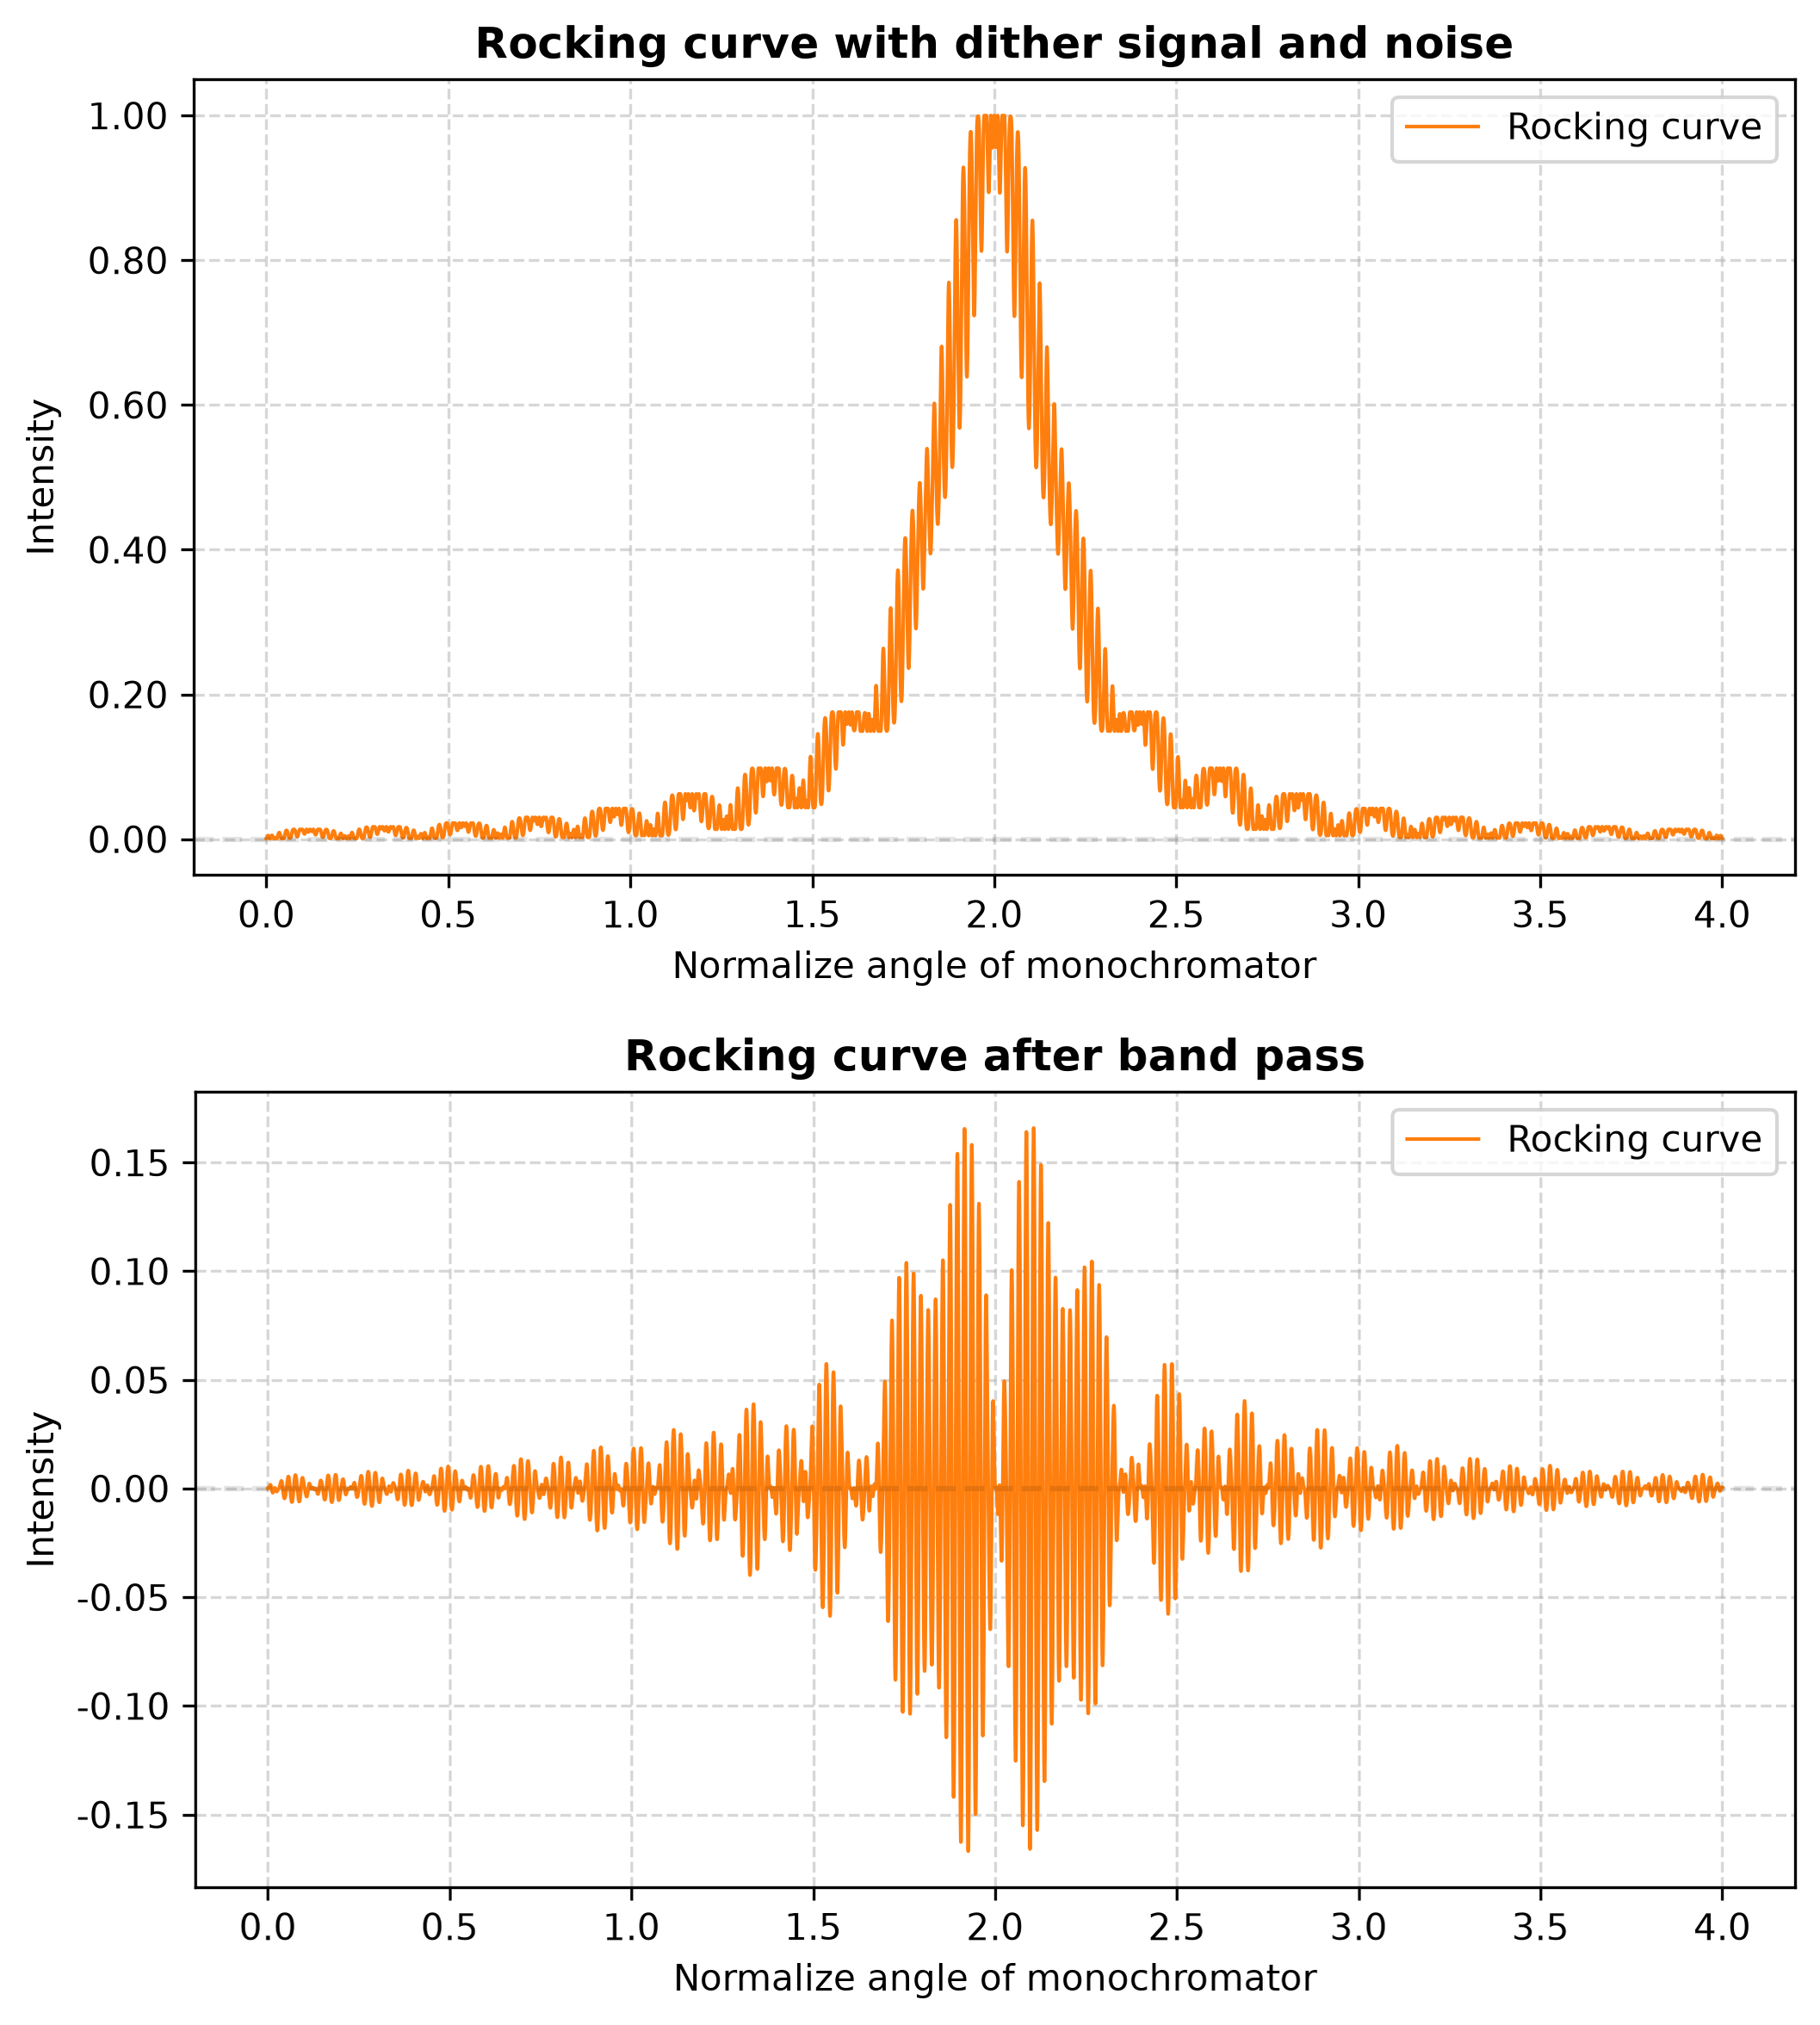
\includegraphics[width=0.85\textwidth]{img/cap 4/band_pass_validation.png}
        \caption{Comparison between before and after bandpass filtering. The input signal was injected with the dither signal and noise.}
        \label{fig:band pass validation}
    \end{figure}
    
    \item \textbf{Second-Harmonic Rejection:}  Mixing the intensity filtered by the pass band with the reference signal, which split the information at frequency $f_d$ into a DC offset and a $2f_d$ component. The mixed signal is then passed through a low pass filter for isolate the DC component which ca be identify in the gradient of the signal useful for the closed-loop integration.
\end{itemize}

\subsection{Gradient Extraction Accuracy ($dI/dt$ Linearity)}
To be analytically certain that the demodulated signal carries the information of the first derivative of intensity, a check was performed with an analytically calculated first derivative on the entire rocking curve, Figure[~\ref{fig:gradient validation}]. 

\begin{figure}[htbp]
    \centering
    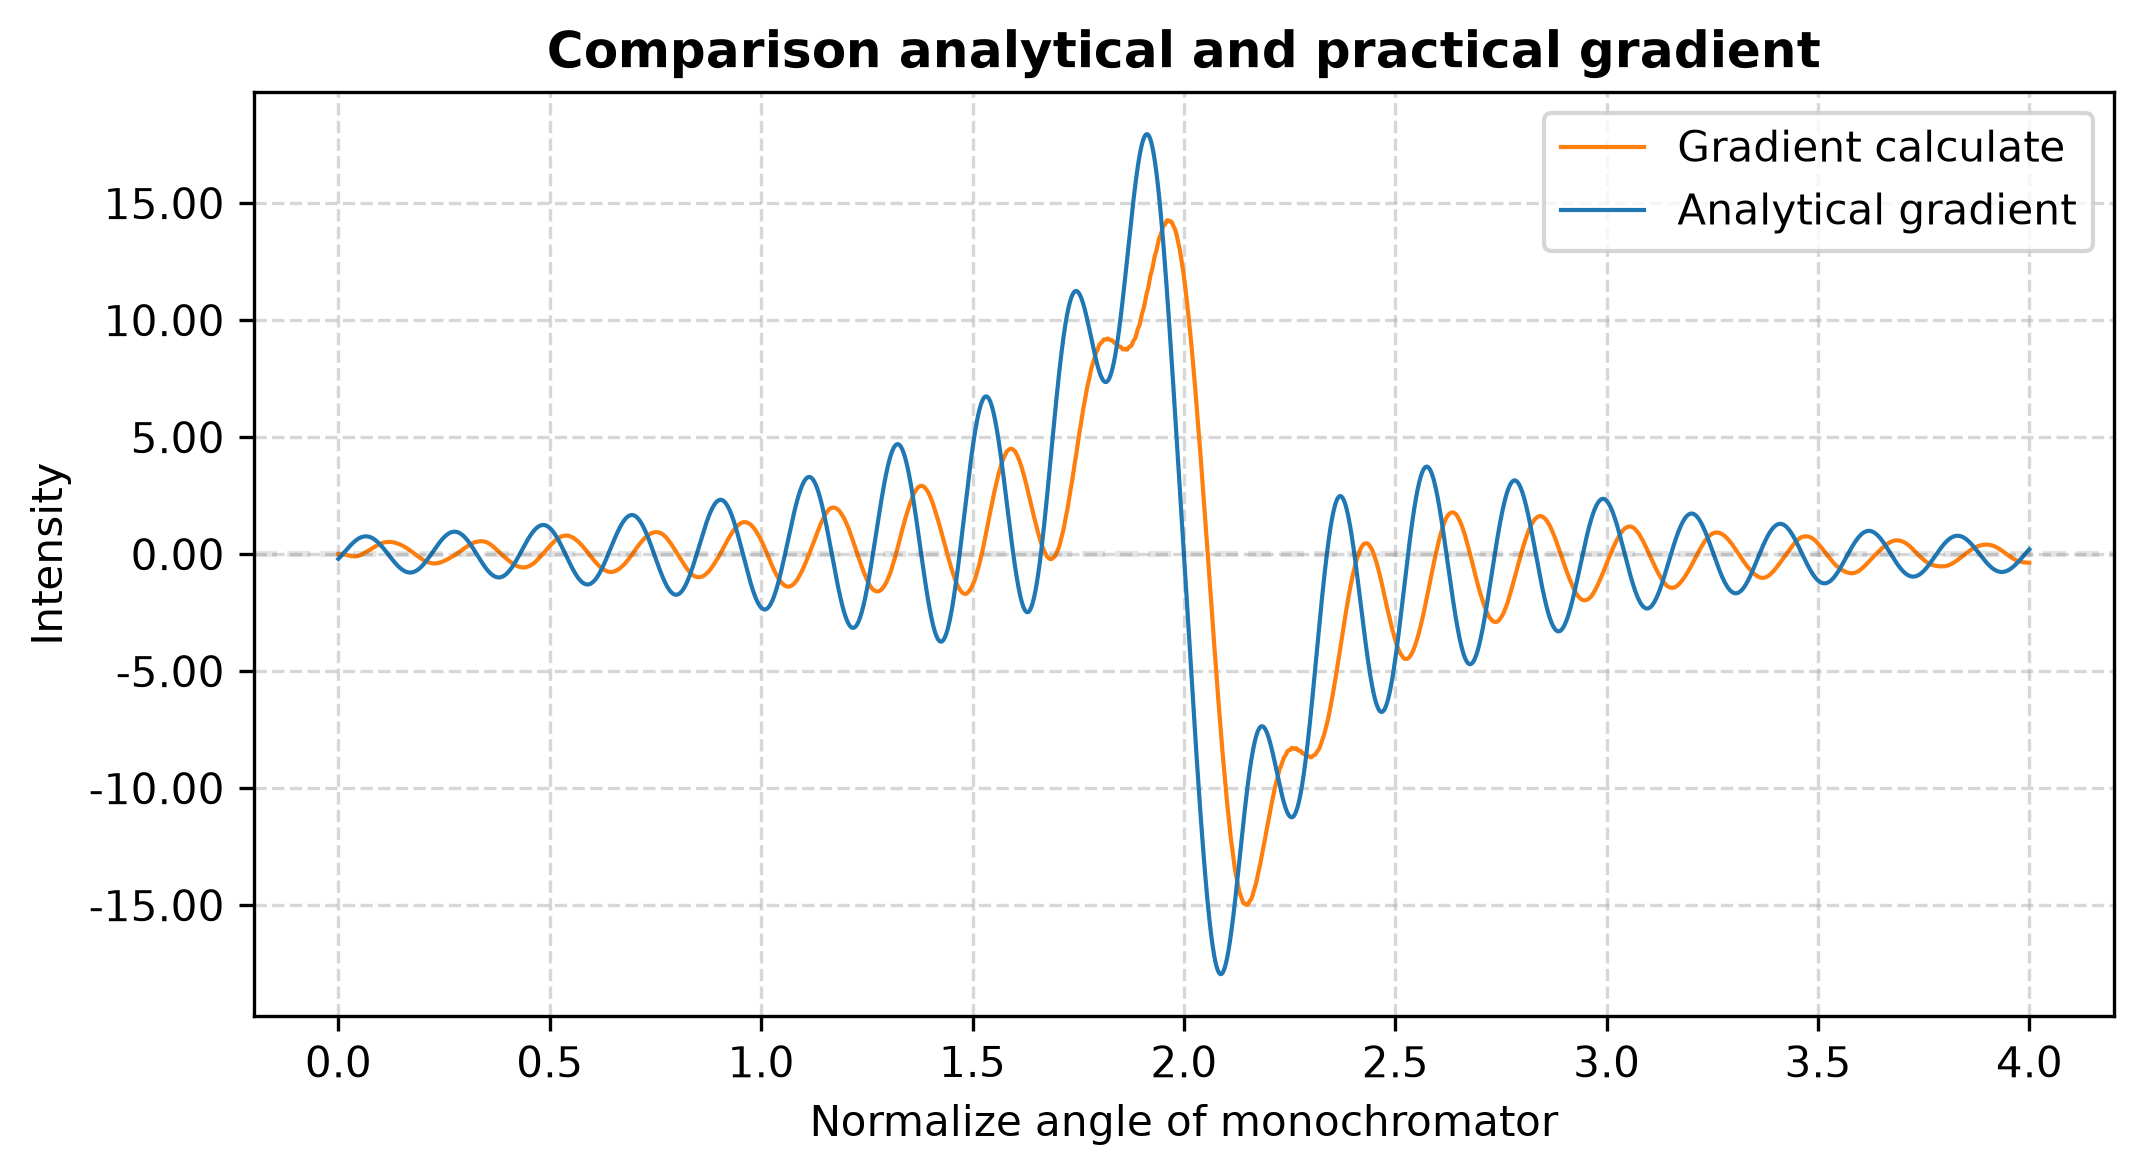
\includegraphics[width=0.85\textwidth]{img/cap 4/Comparison analytical and practical gradient.png}
    \caption{Comparison with the derivative of the simulated rocking curve function and that obtained by moving the monochromator from left to right}
    \label{fig:gradient validation}
\end{figure}

This empirically confirms the correctness of the demodulation procedure. 
Furthermore, just by looking at the graph [~\ref{fig:lockin_stages}] it is possible to distinguish:
\begin{itemize}
    \item \textbf{Zero-Crossing Precision:} The demodulated signal is represented by a classical oscillation centered on zero, which intersects the x-axis at the peak points and which corresponds to the profile of the first derivative of the oscillation curve.
    \item \textbf{Directional Polarity:} Focusing on the peak intensity position $\theta_{\text{peak}}$, if the position it'll slightly shift on the left, it is possible to see the gradient be positive with amplitude higher where the slope is stiffed. While shifting the position on the right, with the same properties, the gradient is negative. Thus the pipeline output shows the ability to recover the gradient of the intensity correctly that it will passed to the feedback controller regardless of which side of the rocking curve the system starts on.
\end{itemize}

\begin{figure}[htbp]
    \centering
    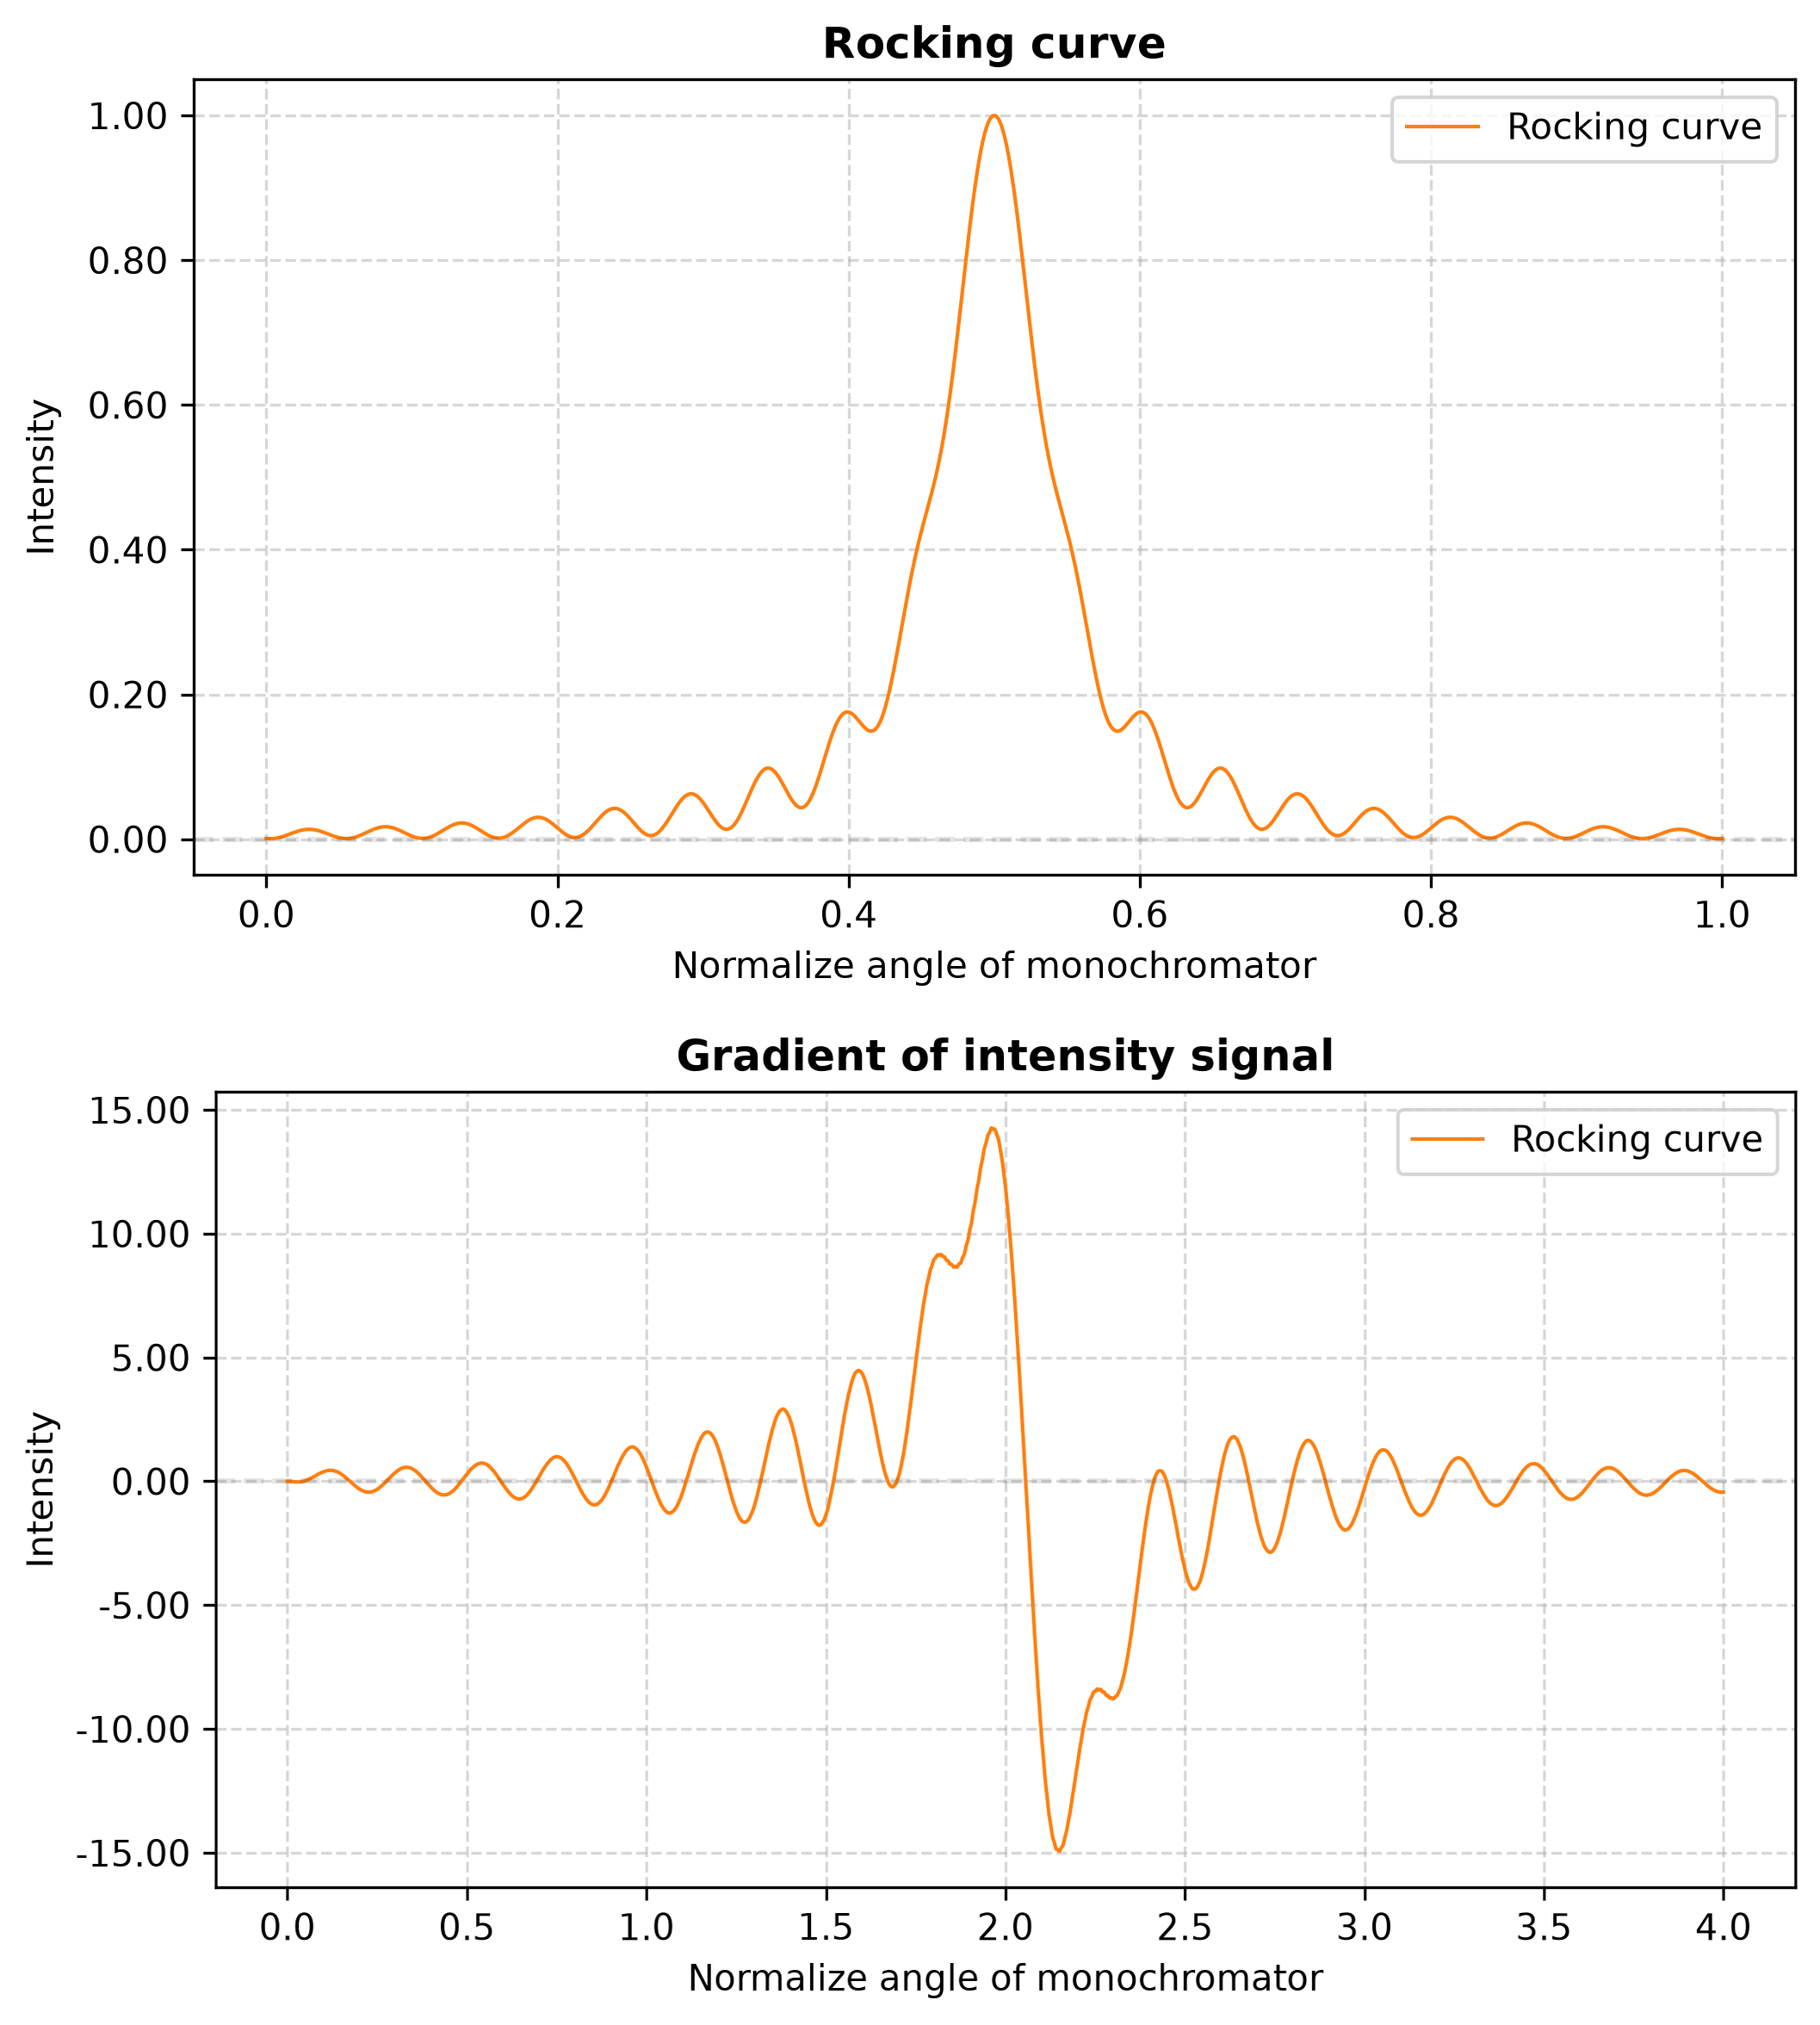
\includegraphics[width=0.85\textwidth]{img/cap 4/rocking curve and gradient calculate.png}
    \caption{Comparison between the simulated rocking curve intensity profile and the extracted lock-in gradient error signal across an angular sweep.}
    \label{fig:lockin_stages}
\end{figure}

\subsection{Steady-State Peak Holding and Dither Amplitude Trade-off}
During a simple simulation excluding all the type of low frequency drift like the thermal one, the controller was able to drive the monochromator to the right position so as to hit the peak of intensity, thus taking the first derivative to zero. 

Tests in this simple environment was useful for understanding the role of $\alpha$ and its trade-off of its magnitude:
\begin{itemize}
    \item \textbf{Small Dither Amplitudes:} 
    If where choose a small amplitude for the dither signal, The advantageous part was having a very small influence on the position by not varying the intensity too much once the peak was reached. On the other hand, however having a small amplitude cause to reduce the signal-to-noise (SNR) ratio, making the system more responsive to noise. An amplitude $\alpha$ is consider small if it is lower than $0.5$ of peak intensity.
    \item \textbf{Larger Dither Amplitudes:} 
    With larger amplitude it work the other way around, the dither signal in this case can make the control system more robust to noise at the cost of a much wider oscillation at the peak intensity once reached.
\end{itemize}
The parameter in this thesis was chosen as a compromise, so as not to have too large oscillations and at the same time not to be excessively sensitive to the noise present in the simulated environment or not.

\section{Automated Phase Calibration and Alignment}

In the previous sub section was establish the correct extraction of the intensity's gradient, but this was obtained under untrue assumptions in a real case.
In fact, in a real case, several additional factors must be taken into account, including the delay caused by the system, which in this case is the beamline.
Taking into account the delay propagation within the control system and the actual movement time of the piezo, this introduces a delay phase ($\phi_{\text{delay}}$) that will have to be managed by the control system as it could affect the gradient extraction performance and thus degrade the effectiveness of the PID.
The reason this delay affects performance is due to the way it interferes between the dither signal and the reference signal.
If the dither signal is applied at time $t$ to the piezoelectric, a certain amount of time $\Delta t$ will pass before it is detected by the BPM. Therefore, if the signal is then demodulated with the reference signal at $t$, the reference signal will be shifted by a time delay of $\Delta t$.
Since this is an instrument that will be used in a variety of settings, creating a way to automate the delay phase calculation process is necessary, using an algorithm instead of manual tuning can reduce the time of implementation of the control system while being less error prone to human error.

\subsection{The Impact of Uncompensated Phase Mismatch}

The reason why this problem was included in the thesis is related to the fact that the demodulation error is scaled with a factor of $\cos(\phi_{\text{delay}})$.
Not taking the phase delay into account can lead to different behaviors of the control system: it could decrease the amplitude of the gradient in the best case, while in the worst case, the error would change sign causing the control system to behave differently than intended.

\subsection{Automated Calibration Procedure and Quadrature Sampling}

The automatic calibration phase of the delay phase is performed early during the start-up phase of the control system, before its main control loop starts.
For simulation purposes the firmware has been modified to make the environment as realistic as possible, the changes made have been minimal and easily removable in order to return to having a firmware ready for use.
The phase delay calibration sequence follow this steps:

\begin{enumerate}
    \item \textbf{Operating Point Initialization:} First, to make the calculation more accurate, the calibration phase should position the monochromator at a point where the gradient neither changes sign nor exhibits a large difference in amplitude when the dither signal is injected. Therefore, the control system sweeps the monochromator across the entire available range, identifying the intensity peak and then positioning itself on one of the two sides.
    \item \textbf{Warm-up and Excitation Window:} Since the phase delay calculation also involves band pass and low pass filtering, the system needs to be warmed up to mitigate the disturbances generated by the initial states of the filters. After the warm-up phase, intensity samples are acquired in a predetermined time window, the sampling window.
    \item \textbf{Simultaneous In-Phase and Quadrature Mixing:} 
    During the whole sampling phase, the acquired intensity is filtered by the band pass and then multiplied by the reference sine wave and an orthogonal reference cosine wave components with frequency $\omega_d$, then both are filtered by the low pass in order to isolate their respective DC levels:
    \begin{align}
        I_{\text{in-phase}}[n] &= I_{\text{bp}}[n] \cdot \sin(\omega_d t_n) \\
        I_{\text{quadrature}}[n] &= I_{\text{bp}}[n] \cdot \cos(\omega_d t_n)
    \end{align}
    \item \textbf{Four-Quadrant Arctangent Computation:} 
    Both DCs of the components will be averaged in order to have a more accurate result, thus the system delay plus the delay injected by the filters is computed by using the four-quadrant arctangent ($\text{atan2}$) function over the mean quadrature and in-phase components:
    \begin{equation}
        \phi_{\text{delay}} = \text{atan2}\left( \frac{1}{N}\sum I_{\text{quadrature}}[n], \, \frac{1}{N}\sum I_{\text{in-phase}}[n] \right)
    \end{equation}
\end{enumerate}

\subsection{Verification of Phase Alignment Accuracy}

Tests have shown that the delay phase calibration routine is able to detect the system delay. Tests were performed with different delay times to make the test more robust.
The phase delay $\phi_{\text{delay}}$ , once calculated, will then be used by the reference signal to realign it to the dither signal.

For reference, simulations were performed with delays in the system without correcting the phase and the degradation of the control system was demonstrated.
Thanks to the calibration sequence, the reference signal is able to correctly demodulate the intensity signal having the error phase close to zero.
This also helped with system stability once the control system was up and running.

\section{Convergence Dynamics and Disturbance Rejection}

After having demonstrated the correctness of the individual phases of the pipeline and that the calculation of the delay phase was correct, it is now possible to investigate the control system as a whole and investigate the convergence to the peak intensity by testing.
Going into detail, this section also deals with the mechanical friction of the Double Crystal Monochromator (DCM) actuators and the thermal displacement.
The convergence test also includes these factors as they are the motivation that led to the beginning of this thesis.

\subsection{Closed-Loop Acquisition and Convergence Time}
In a real case scenario when the control loops is enable the starting point is already on the peak, because the main purpose of the control system is to maintain the peak intensity, but for testing the convergence in a static case where the rocking curve does not shift the start position was modified. 
It start from half from one side of the peak of intensity, so as to be equidistant from the main peak and the lateral peaks:
\begin{enumerate}
    \item \textbf{Gradient-Driven Trajectory:} The demodulated signal provide the gradient of the intensity signal and provide the direction for the controller. At each iteration, the PID attempts to adjust the position of the monochromator by applying a control signal to the piezoelectric element. The goal of the PID is to drive the piezoelectric element so as to cancel the gradient ($\text{d}I/\text{d}\theta = 0$).
    \item \textbf{Settling Behavior and Overshoot:} Tuning the parameter of the PID ($K_p,K_i,K_d$) was made manual with a try-and-error approach, they where choose in a way to have a controller to converge fast and guarantee stability once the peak is reached.
    As mention before in simulation telemetry, the control system reach convergence at time of [~\ref{fig:feedback control loop response}] it stabilizes cautiously with a slight initial overshoot without endlessly oscillation or trying to achieve its goal even once reached.
\end{enumerate}

\begin{figure}[htbp]
    \centering
    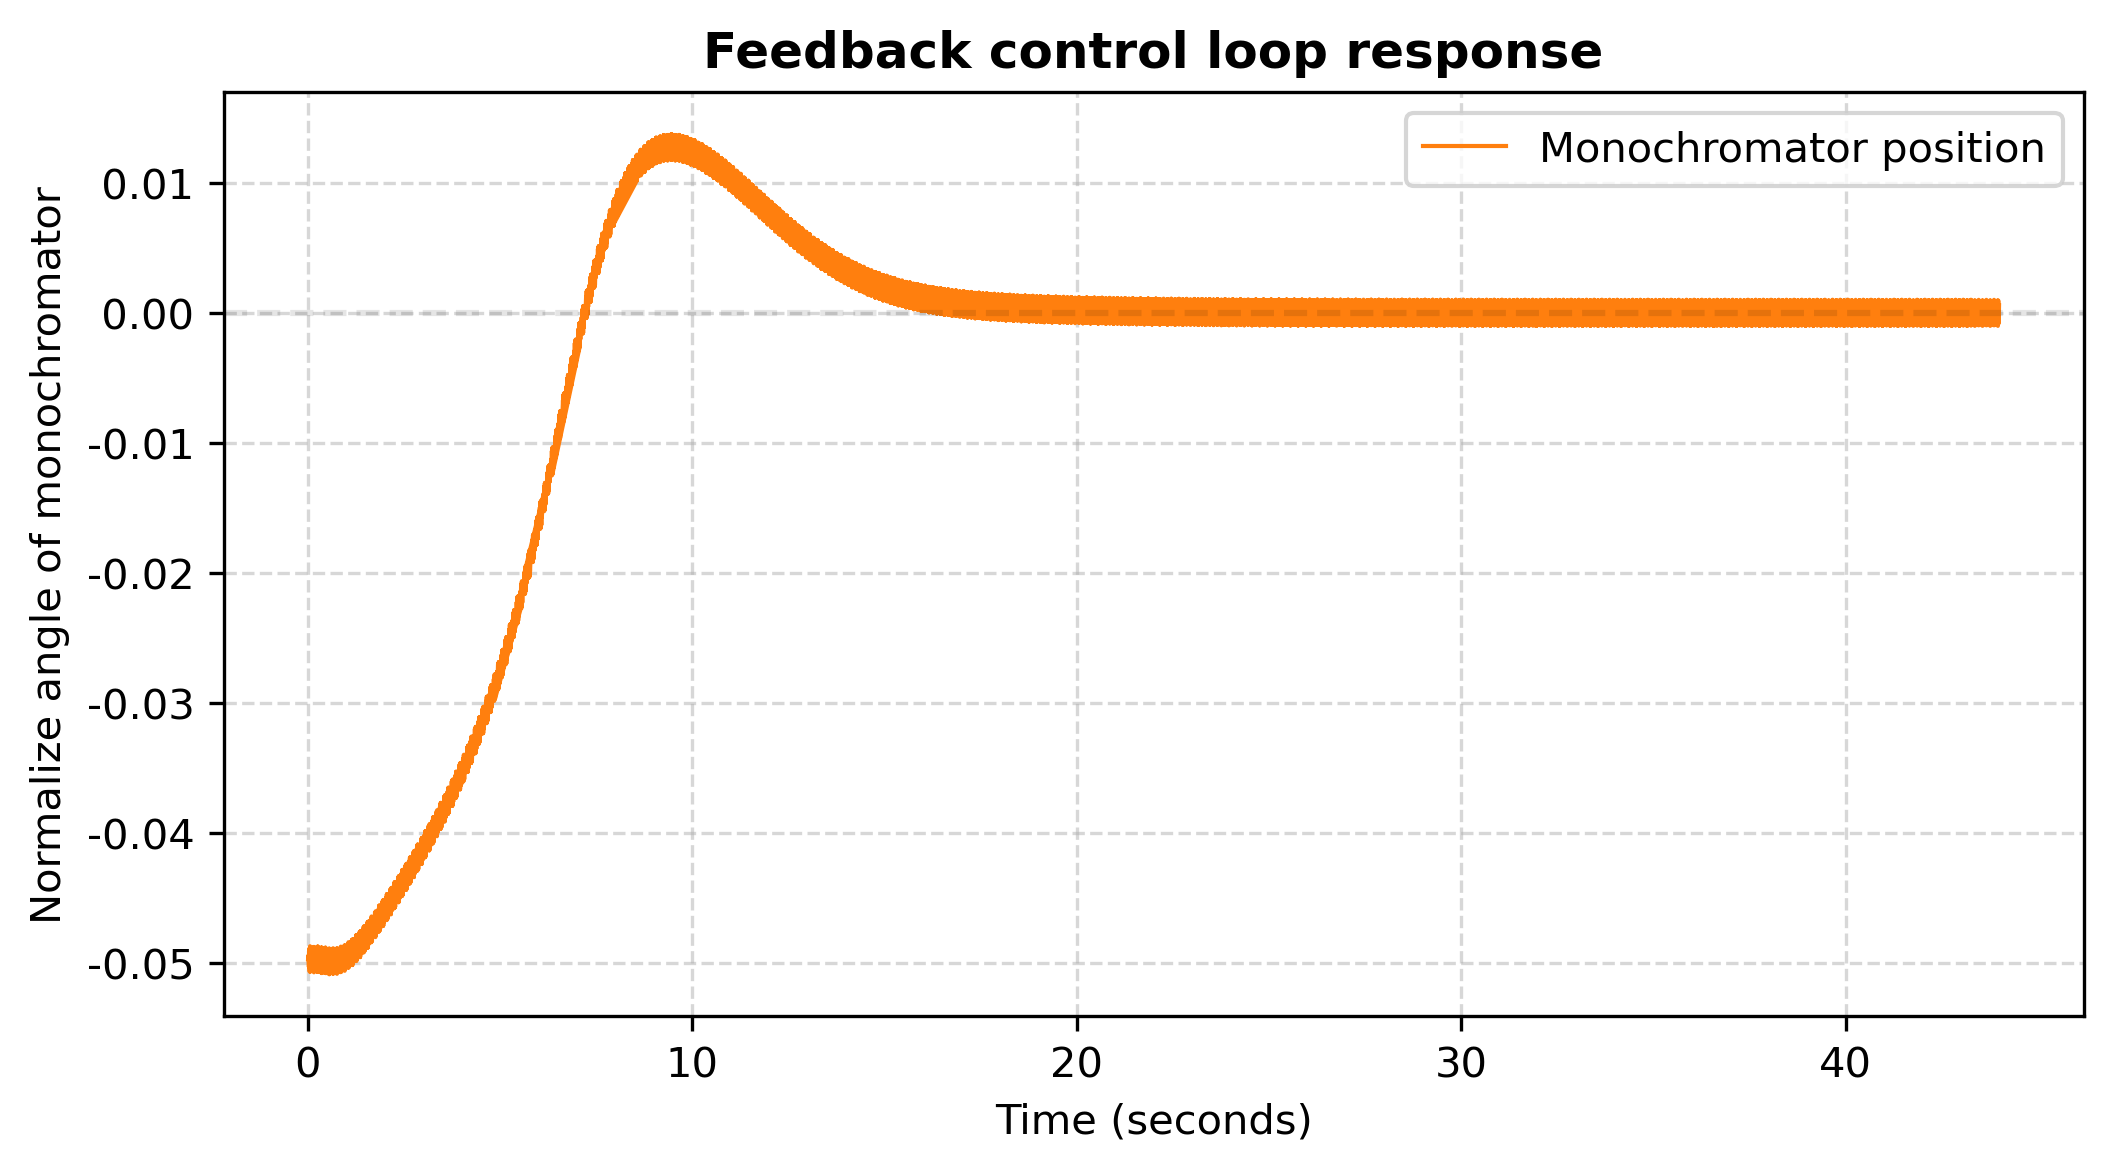
\includegraphics[width=0.85\textwidth]{img/cap 4/Feedback control loop response.png}
    \caption{Controller response to reach set point when monochromator is at position -0.045.}
    \label{fig:feedback control loop response}
\end{figure}

\subsection{Thermal and Mechanical Disturbance Rejection}

Optical component inside a real synchrotron beamline, during long experiments the crystal lattice can expand or contract if change its temperature. 
This leads to a shift in the rocking curve and consequently to a shift in the intensity peak.
To emulate the thermal displacement component, it must be translated into a time-varying displacement. 
Knowing that thermal drift is a low-frequency phenomenon, the equation describing the thermal displacement for the simulation is a sine wave with frequency of $0.001\text{kHz}$, so the peak of the rocking curve shifts by the sine wave.

\begin{itemize}
    \item \textbf{Tracking Drift Dynamics:} 
    If not taken into account, thermal drift causes a loss of beam intensity as the peak moves away from the position of the monochromator which instead remains stationary.
    \item \textbf{Closed-Loop Compensation:} 
    Instead, if the control system is activated, it is able, as has already been demonstrated, to detect the variation in the derivative of the intensity.
    The PID controller, receiving the derivative of the intensity, calculates the amount of movement needed by the piezoelectric to continue following the migrating peak and must do so for extended periods of operation, maintaining stability at the peak intensity.
\end{itemize}

\begin{figure}[htbp]
    \centering
    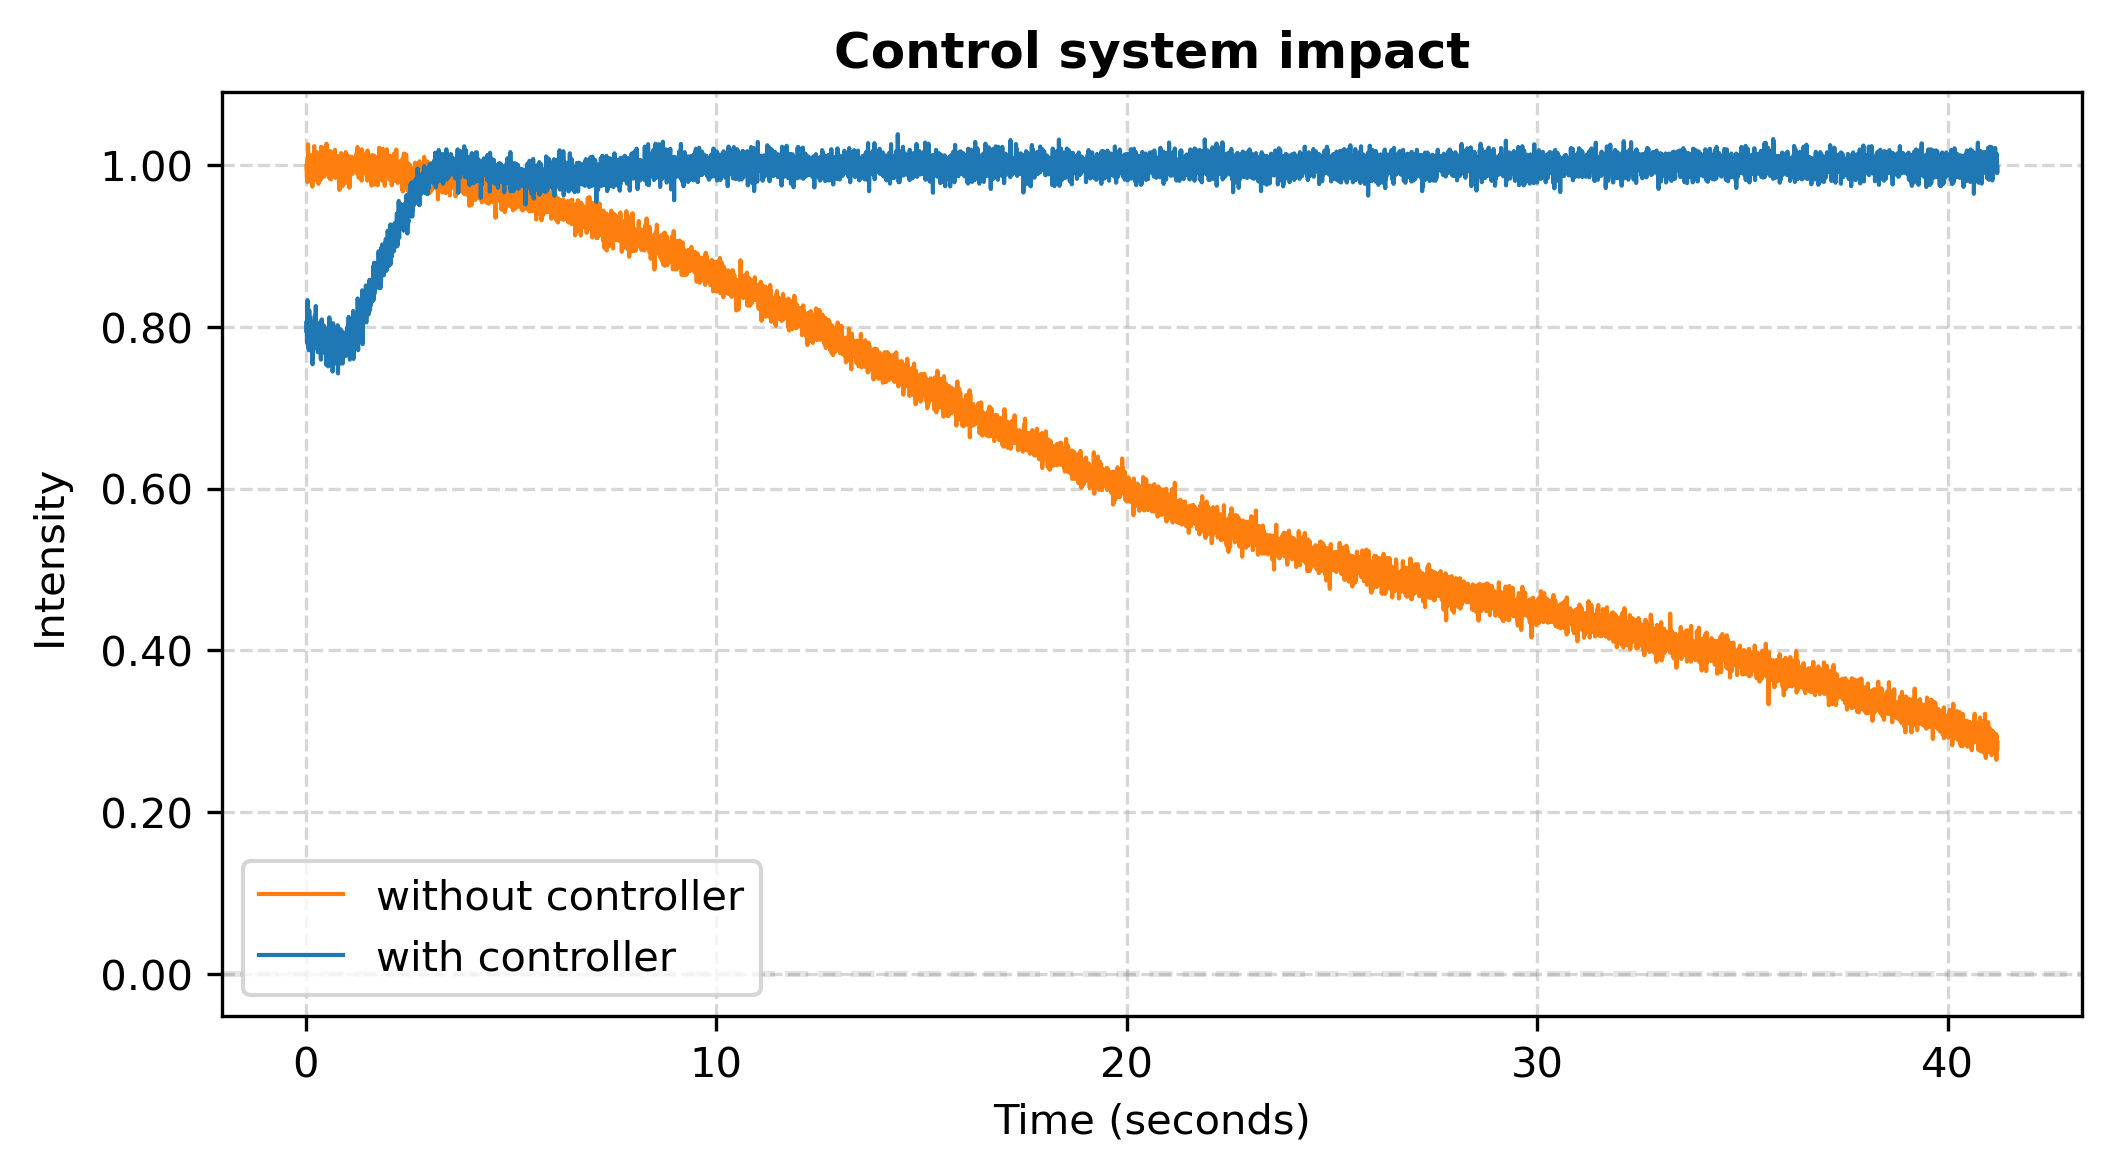
\includegraphics[width=0.85\textwidth]{img/cap 4/Control system impact.png}
    \caption{The impact of the control system in case of noise and thermal drift against keeping the monochromator position fixed.}
    \label{fig:disturbance_rejection}
\end{figure}

\subsection{Steady-State Stability and Jitter Analysis}

Once peak intensity was reached, the control system demonstrated robust steady-state stability.
Even if the controller reach his set point, control signal still will not be zero due to the dither amplitude ($\alpha$) and the low-pass filter bandwidth.

Since the main circuitry of the control system is executed within the FPGA using an interrupt service routine (ISR), the control is called at deterministic intervals, thus eliminating jitter.
The interrupt service routine is triggered by a signal emitted at a frequency of $100\text{ kHz}$.

\section{Driver Telemetry and Supervisory GUI Verification}

To be able to view the internal behavior of the control system through parameters such as the intensity derivative, the control signal, or the intensity itself, it was necessary to extract the telemetry data and implement an interface to display them.
Based on the existing implementation of communication between the FPGA and the host PC, which operates via a shared map memory, it was possible to use some unreserved slots for extracting telemetry data.
Although a graphical implementation for displaying telemetry data was already available, it was necessary to build another framework to analyze this data more practically, as Python is easier for data analysis than the Qt framework for C/C++.

\subsection{Python-Based Telemetry and Pipeline Analysis Framework}

Another rejected solution was to debug within the Quartus II development environment, but this presented significant debugging constraints, so a parallel testing pipeline was constructed in Python:
\begin{itemize}
    \item \textbf{Data Logging and Export:} 
    By making the data available in memory, it was sufficient to find the indexes whose slots were reserved for the simulation data. The calls to read the data were performed using an already developed library.
    \item \textbf{Online Validation:}  The data analysis was performed after a visual validation of the control system behavior inside a control panel, which helped in the implementation phase of the FPGA and the tuning of the parameters present within the control system. Figure[~\ref{fig:monitoring panel}]

\begin{landscape}
\begin{figure}[p]
    \centering
    \includegraphics[
        width=\linewidth,
        height=0.85\textheight,
        keepaspectratio
    ]{img/cap 4/Monitoring panel.png}
    \caption{Control panel for monitoring the control system under development, with access to specific memory slots.}
    \label{fig:monitoring panel}
\end{figure}
\end{landscape}
    
    \item \textbf{Offline Validation and Plotting:} 
    Before implementing the solution on the FPGA, it was simulated and tested in a more practical environment to make the implementation cleaner once the results were obtained.
    Python was useful because the easy modifications to the code led to faster development and the ability to create graphs using scientific packages (such as NumPy, SciPy, and Matplotlib).
    It was also useful for calculating the coefficients of the bandpass and lowpass filters.
    Furthermore, the framework for real-time visualization of the simulation on the FPGA made it possible to acquire the data for the analyses mentioned in the previous sections.
\end{itemize}

\subsection{Supervisory GUI Integration and Real-Time Visibility}
For a real-world implementation of the system at a physical facility, the framework created in Python cannot be used, as its purpose is only to simulate the physical system.
The local GUI already developed in Qt C++ performs various functions for monitoring and tuning the control system previously developed for position control:
\begin{itemize}
    \item \textbf{Real-Time Gradient and Rocking Curve Rendering:} 
    The GUI already provides the ability to view various system parameters such as the position of the beam and its intensity, now in addition, it is possible to observe the trend of the first derivative, giving operators immediate visual confirmation of whether the system is locked onto the peak.
    \item \textbf{Dynamic Parameter Configuration:} 
    Through a communication channel other than shared memory, the mailbox allows information to be shared between the host PC and the FPGA. This communication channel was designed to avoid the need to continuously send data, as happens with shared memory, for example.
    In the mailbox, it is used to set the parameters of the PID used for position control.
\end{itemize}

\begin{landscape}
\begin{figure}[p]
    \centering
    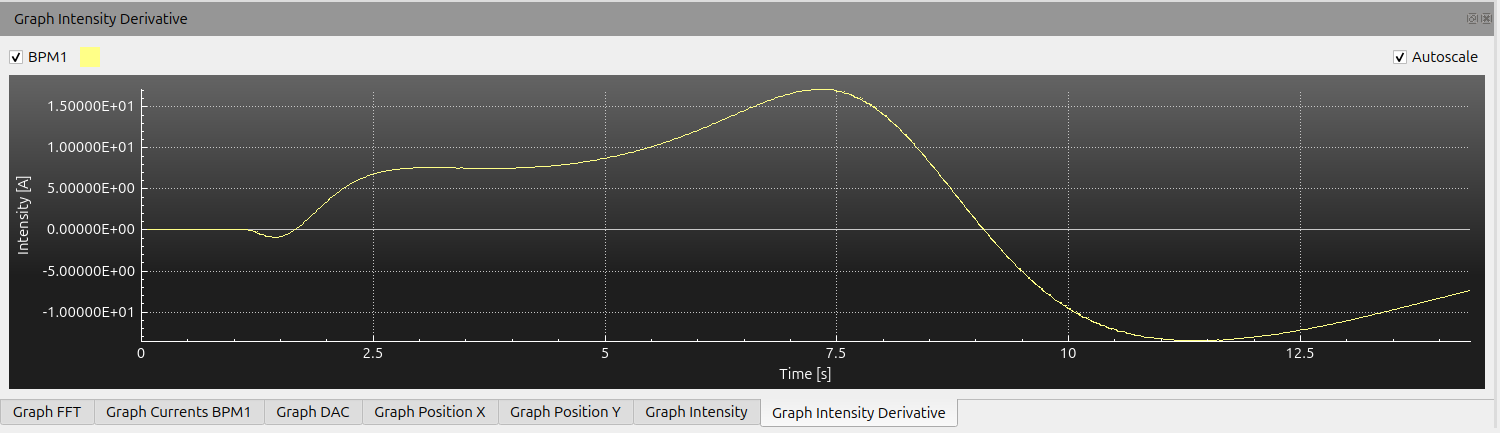
\includegraphics[
        width=\linewidth,
        height=0.85\textheight,
        keepaspectratio
    ]{img/cap 4/local GUI.png}
    \caption{Prototype of the integrated monitoring interface within the local Qt/C++ GUI.}
    \label{fig:disturbance rejection}
\end{figure}
\end{landscape}

Through a communication channel other than shared memory, the mailbox allows information to be shared between the host PC and the FPGA. This communication channel was designed to avoid the need to continuously send data, as happens with shared memory, for example.
In the mailbox, it is used to set the parameters of the PID used for position control.

\section{Summary of Validation Results}

The proposed system was tested to validate it and demonstrate its capability in maintaining the monochromator position that corresponds to the maximum beam intensity.
Testing the system in a real case scenario proved impractical, as the synchrotrons using the equipment are few and not always available.
So instead of having a real plant for the tests, it was simulated by mocking the FPGA input intensity.
In this way it was possible to test the system under different circumstances by adding noise, phase delay and thermal drift.

Before going to test the system behavior, it was necessary to analyze the FPGA implementation to ensure that it respected the execution time and memory constraints.

Afterwards, the individual stages of the pipeline were analyzed to verify that each of them performed its task correctly.
The results showed the correct filtering of the bandpass filter by isolating the dither signal, and the demodulation led to a correct extraction of the intensity gradient.

Even if all the stages taken alone were proven correct, in real case scenario the pipeline might not work because it doesn't take the system's delay time into account. 
if it is not taken into consideration, there's a risk that demodulation will be incorrect.
Tests have demonstrated the correct calculation of the phase delay.

The control system correctly identified the direction to take to adjust the monochromator's position to follow the intensity peak. 
Furthermore, the PID was tuned to achieve the desired behavior and it was demonstrated its stability once the maximum was reached, even when thermal drift was present. 
Tests on the control system concluded by comparing it with a system operating without feedback, showing showing the advantage of having an active peak tracking system.

The tests were accompanied by a control panel built specifically for the tests, which allowed monitoring the intermediate stages of the control system. Meanwhile, the intensity gradient display was integrated into the local GUI.

The results demonstrated the validity of the proposed solution implemented inside the FPGA.
However, this control system should be tested with a real plant, in order to verify its behaviour under real operating conditions.

\newpage

%*******************************************************
% Capitolo conclusivo
%*******************************************************
\chapter*{Conclusioni}
% Non modificare questa parte
\addcontentsline{toc}{chapter}{Conclusioni}
\label{chap:concl}
\markboth{CONCLUSIONI}{CONCLUSIONI}
% Non modificare questa parte

Beamlines can have problems to continuously hit the intensity peak.
The problem of not always hitting the peak can be caused by many factors, including thermal drift and mechanical friction.
In the thesis, a solution was proposed for the ELS Instruments in which a control system tracks the peak intensity of the photon beam. 
The proposed solution will be integrated into the BEST system, which aims to support synchrotron facilities.
Specifically, the solution was designed to counteract the thermal drift of the DCMs, which cause beam intensity degradation.
The BEST, starting with only beam position control, is unable to detect and compensate beam intensity degradation, therefore, to overcome this problem, it was necessary to modify the instrumentation already implemented at firmware level. 
Changes have been made to accommodate the new solution, the were heterogeneous within the instrumentation as it is composed of different components; the modifications included parts of the FPGA, the NIOS II soft processor, and the local GUI.
The implementation added the following features to the BEST system:

\begin{itemize}
    \item \textbf{A Four-Stage Digital Lock-in Pipeline:} 
    The main component of the work is the pipeline for extracting the beam intensity gradient, which includes, in this order: a bandpass filter, demodulation, a lowpass filter, and a PID controller.
    \item \textbf{Automated Startup Phase Calibration:} 
    To ensure correct demodulation it is necessary to calculate the delay induced by the system in which the instrumentation will be implemented.
    Since the delay varies depending for each system, it was necessary to create a delay calculation routine, based on in-phase sampling and quadrature combined with a four-quadrant arctangent calculation ($\text{atan2}$).
    \item \textbf{Software-in-the-Loop (SIL) Validation:} 
    To test the solution, an internal simulation of the system was proposed. This led to rapid development of the tests and the ability to adapt them if necessary. So it was possible to test different dynamics of the solution and different rocking curves from the static to the dynamic one.
\end{itemize}

\section{Achievement of Thesis Objectives}

The main objective of the thesis was to build a peak tracking system based on solution already reviewed.
The system built will counteract the shifts effect caused by thermal drift.

During the testing phase, the solution was shown to be able to extract the intensity gradient and provide the correct error signal to the PID controller. 
The tests also covered the phase delay calibration routine, which also passed successfully. This demonstrated that the control system is capable of compensating for the delay introduced by the system.

Tests that included simulation demonstrated the system's ability to track the peak over time, even when thermal drift was added. It also demonstrated stable intensity, which would not be the case without control.

The results demonstrated that the primary objective of the thesis was achieved.

\section{Comparison with the MoCo Controller}

The proposed solution shares the same core idea as MoCo developed by ESRF \cite{MoCo2008}.
Both use the intensity gradient as information to adjust the angle of the monochromator.


Although they share the same principle, the implementation is different.
MoCo is a dedicated controller while what was done in this thesis is an addition to an already functioning system.
MoCo uses an integrator as its controller, while the proposed solution uses a full PID.
A full PID gives more freedom over the controller's behavior and can still be used as an integrator.
Another difference is in the phase delay calculation: MoCo allows for manual setting, while in the thesis it is calculated automatically using a routine. The procedure itself is based on in-phase and quadrature sampling.

Therefore, the solution was created by drawing inspiration from various sources, including the MoCo manual, for its implementation within the BEST system.
This meant extending the functionality of BEST by adding peak intensity tracking control to the existing position tracking control.

\section{Future Developments and Research Directions}
The proposed solution has been shown to be capable of fulfilling its duties of tracking in real time the peak intensity, several avenues can be taken to expand on what has already been done in this thesis from future research to make it more customizable according to needs.

\begin{itemize}

    \item \textbf{Continuous Phase Calibration:}
    The phase delay is calculated only once at the start of the control system.
    The assumption that the delay introduced by the system remains constant, especially during long-time operations, could be false due to thermal expansion of cables, amplifiers, and mechanical linkages. Therefore, once calculated at startup, the phase delay should be tracked on the fly without interrupting beam delivery to maintain correct demodulation.

    \item \textbf{Runtime Parameter Configuration:}
    The solution implemented in this thesis has coefficients written directly into the firmware without the possibility of being modified, such as for example the PID frequency (fixed at $100\text{ Hz}$) and the IIR filter coefficients.
    A possible continuation of the project would be to use the local GUI to modify the configuration parameters and calculate IIR filters coefficients depending on the system dynamics.
\end{itemize}

%*******************************************************
% Appendice
%*******************************************************
% Non modificare questa parte
\pagestyle{fancy}
\renewcommand{\chaptermark}[1]{\markboth{\MakeUppercase{APPENDICE\ \thechapter.\ #1}}{}}
% Non modificare questa parte

\appendix\label{appendix}

\chapter{Sit Amet}

\lipsum[1]

\section{Lorem Ipsum}
\lipsum[2-4]

\subsection{Dolor sit amet}
\lipsum[5-7]
\chapter{Sit Amet}

\lipsum[1]

\section{Lorem Ipsum}
\lipsum[2-4]

\subsection{Dolor sit amet}
\lipsum[5-7]
\chapter{Lorem}

\lipsum[1]

\section{Lorem Ipsum}
\lipsum[2-4]

\subsection{Dolor sit amet}
\lipsum[5-7]

\backmatter

%*******************************************************
% Bibliografia
%*******************************************************
\nocite{*}
\bibliography{Bibliografia}
\bibliographystyle{plain}

%*******************************************************
% Dedica finale o ringraziamenti
%*******************************************************
% Non modificare questa parte
\chapter*{}
\thispagestyle{empty}
\vspace*{3cm}
% Non modificare questa parte

\begin{center}
\hfill Ei fu. Siccome immobile, \\
\hfill Dato il mortal sospiro, \\
\hfill Stette la spoglia immemore \\
\hfill Orba di tanto spiro \\ \medskip
\hfill Alessandro Manzoni -- \emph{Il Cinque Maggio}
\end{center}

\end{document}